\definecolor{aliceblue}{rgb}{0.94, 0.97, 1.0}
\chapter{Experimental Details and Results}
\label{chap:experimentals-details-and-results}
\textit{This chapter describes the experimental results and their interpretation by using a model based on the breakdown $T_d$ symmetry.}
\vfill
\minitoc
\newpage

\section{Samples Description}
\label{sec:chapter-3-section-samples-description}
\vspace{-10mm}
\lettrine[lines=3, lraise=.1, nindent=0mm, slope=0mm]{\textbf{Q}}{uantum structures} 
% were created thanks to the technic Molecular Beam Epitaxy (MBE) growth which in general terms consist in great precision of the growing thin films of semiconductor materials, through high precision  deposition on a suitable  crystalline substrate. As has been pointed out on many occasions, MBE  is nothing more than a sophisticated form of vacuum evaporation\footnote{In owner  experience, MBE growth is a very exhausting task, so great respect to all people that works on this}\cite{orton2015molecular}, this does not sound bad but the MBE technique is not only this, epitaxial growth needed  the precision in experimental  growth parameters how temperature, deposition rate calculations, REED analysis, etc. So that in a bit of words the purpose is to  supply appropriate atoms or molecules to the substrate surface and leave surface diffusion, surface reactions and inevitable desorption from the surface to play their various roles in generating an epitaxial film\cite{orton2015molecular,grundmann2010physics}. 
were fabricated by Molecular Beam Epitaxy (MBE) which consists in great precision of the growing thin films of semiconductor materials on a suitable crystalline substrate. As has been pointed out on many occasions, MBE is
nothing more than a sophisticated form of vacuum evaporation\footnote{In owner  experience, MBE growth is a very exhausting task, so great respect to all people that works on this} \cite{orton2015molecular}, this does not sound
bad but the MBE technique is not only this, epitaxial growth needed the precision in experimental growth parameters how temperature, deposition rate calculations, RHEED analysis, etc.\cite{orton2015molecular,grundmann2010physics}.

\begin{figure}[H]
	\centering
	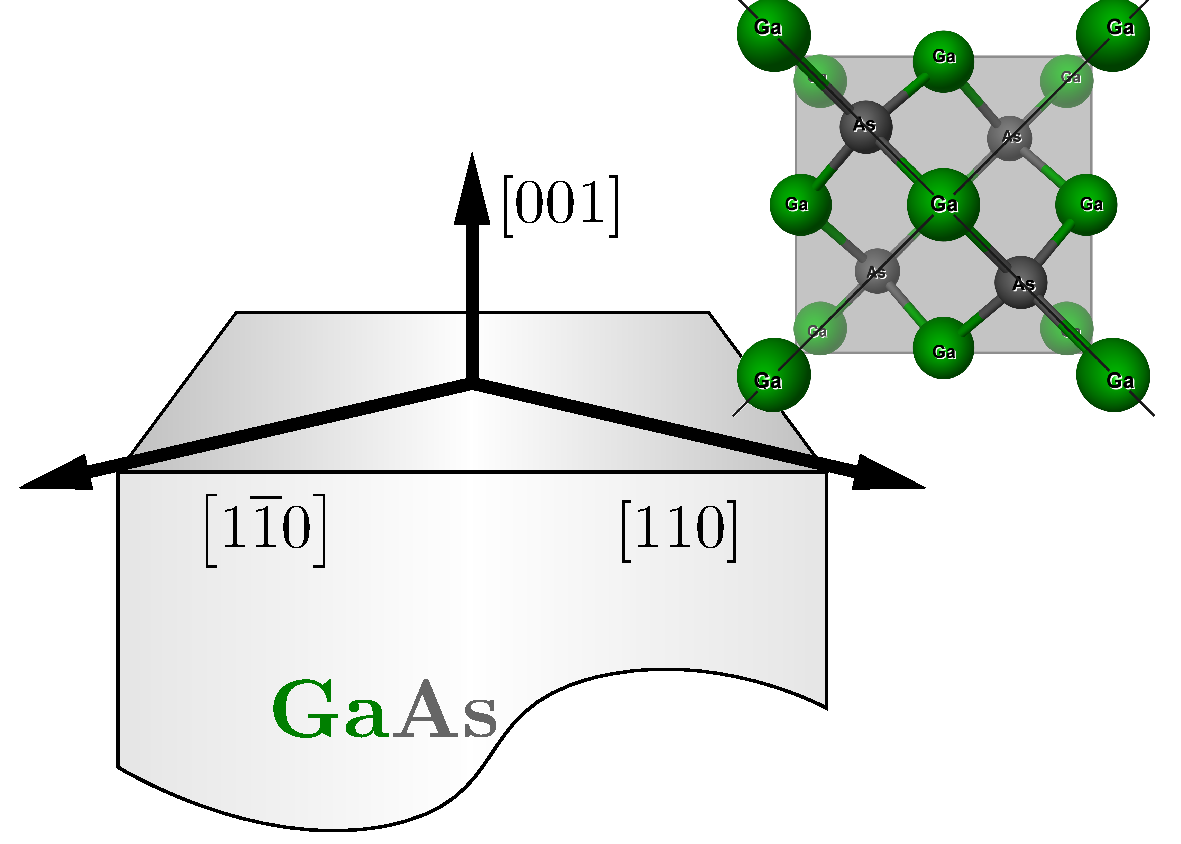
\includegraphics[width=0.7\textwidth]{../figures/chapter-3/crystal-1/build-ruco/crystal-1.pdf}
	\caption[GaAs substrate growth direction]{GaAs (001) substrate. The inset shows the atomic arrangement on the surface with no reconstruction.}
	\label{fig:chapter-3 GaAs Substrate}
\end{figure}

The samples studied in this work, are made up of a GaAs (001) substrate, the GaAs substrate has a zincblende-type crystal structure, in which the atoms are tetrahedrally coordinated \Cref{fig:chapter-3 GaAs Substrate} the choice of crystal is very important and preparation of these can modify the growth result, for this reason, the high quality of substrate is the basis of growth of heterostructures. The heterostructures are a combination of more than one semiconductor, this leads to the superlattice definition where more of two semiconductors are atomically deposited over the substrate in the growth direction (001).  The semiconductors used in the samples are GaAs and AlAs then these can have different thicknesses, growing periodic as how grid and alternately way over the substrate with thickness $d_{\GaAs{\scriptsize}}+d_{\AlAs{\scriptsize}}$. The result consists in an arrangement of $(\GaAs{\normalfont})_{2}\,(\AlAs{\normalfont})_{2}$ superlattice,  like a  shown in  \Cref{fig:chapter-3 AlGaAs Cell} or AB arrangement like a said commonly. In QWs structures, the width is the principal characteristic because quantum confinement is dependent on this, then MBE is the perfect choice to realize this.  


\begin{figure}[H]
	\centering
	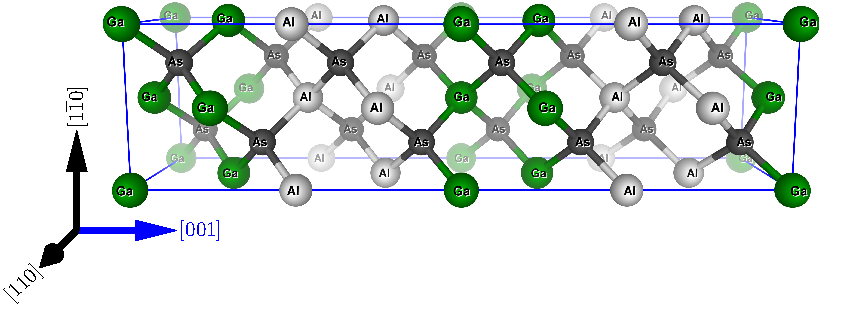
\includegraphics[width=\textwidth]{../figures/chapter-3/crystal-2/build-ruco/crystal-2.pdf}
	\caption[AlGaAs superlattice]{Atomic order in AlGaAs crystal structure grown  along (001) direction. }
	\label{fig:chapter-3 AlGaAs Cell}
\end{figure}

The realistic structures present some details that can modify the experimental results, some of these are inevitability due to the complexity of growth. One of these is the interfaces between two different materials, i.e., the typical structure of GaAs/AlGaas has an interface between these, then the problem is due to an imperfect mismatch of materials, therefore, can cause anisotropy effects. Other details which usually are considered are surface, point defects along of structure, or strained caused by over layer in the epitaxial process.  Later, the interfacial detail gives the physical sense to RAS experiments in the symmetric CQWs structures. 

\Cref{tab:chapter3:Samples description} shows the sample names, each sample has two QWs coupled by a thin barrier preferentially of \algaas semiconductor where Al percent is important because of the barriers potentials depends on this, in the case of AlAs barriers the potential barrier is bigger than \algaas. As a before-mentioned, this was taken into account in numerical calculations to generate the potential profile. Commonly for the case, \algaas barriers both in adjacent like the coupling barrier the $x$ values are in the interval $0.1<x<0.4$.\\*
It is worth mentioning that the purpose of the first four samples (up to down in table) is that they
were grown with the aiming to measure indirect excitons (\gls{ix}), and hence the structures
are more complex, and we omitted the value of n-doped since these samples are doped
in both  bottom and top to minimize the intrinsic electric field (screening field effect), so that
external perturbation is applied through a voltage over the sample\cite{yuan2018tunneling} and the n-doped
enhance the external perturbation\footnote{Non-published, the specific information about the doped  in these growths, if you have a question about this, you can send email to Dr. Klaus Biermann \url{biermann@pdi-berlin.de}}.

\begin{landscape}
	\begin{table}
		\centering
		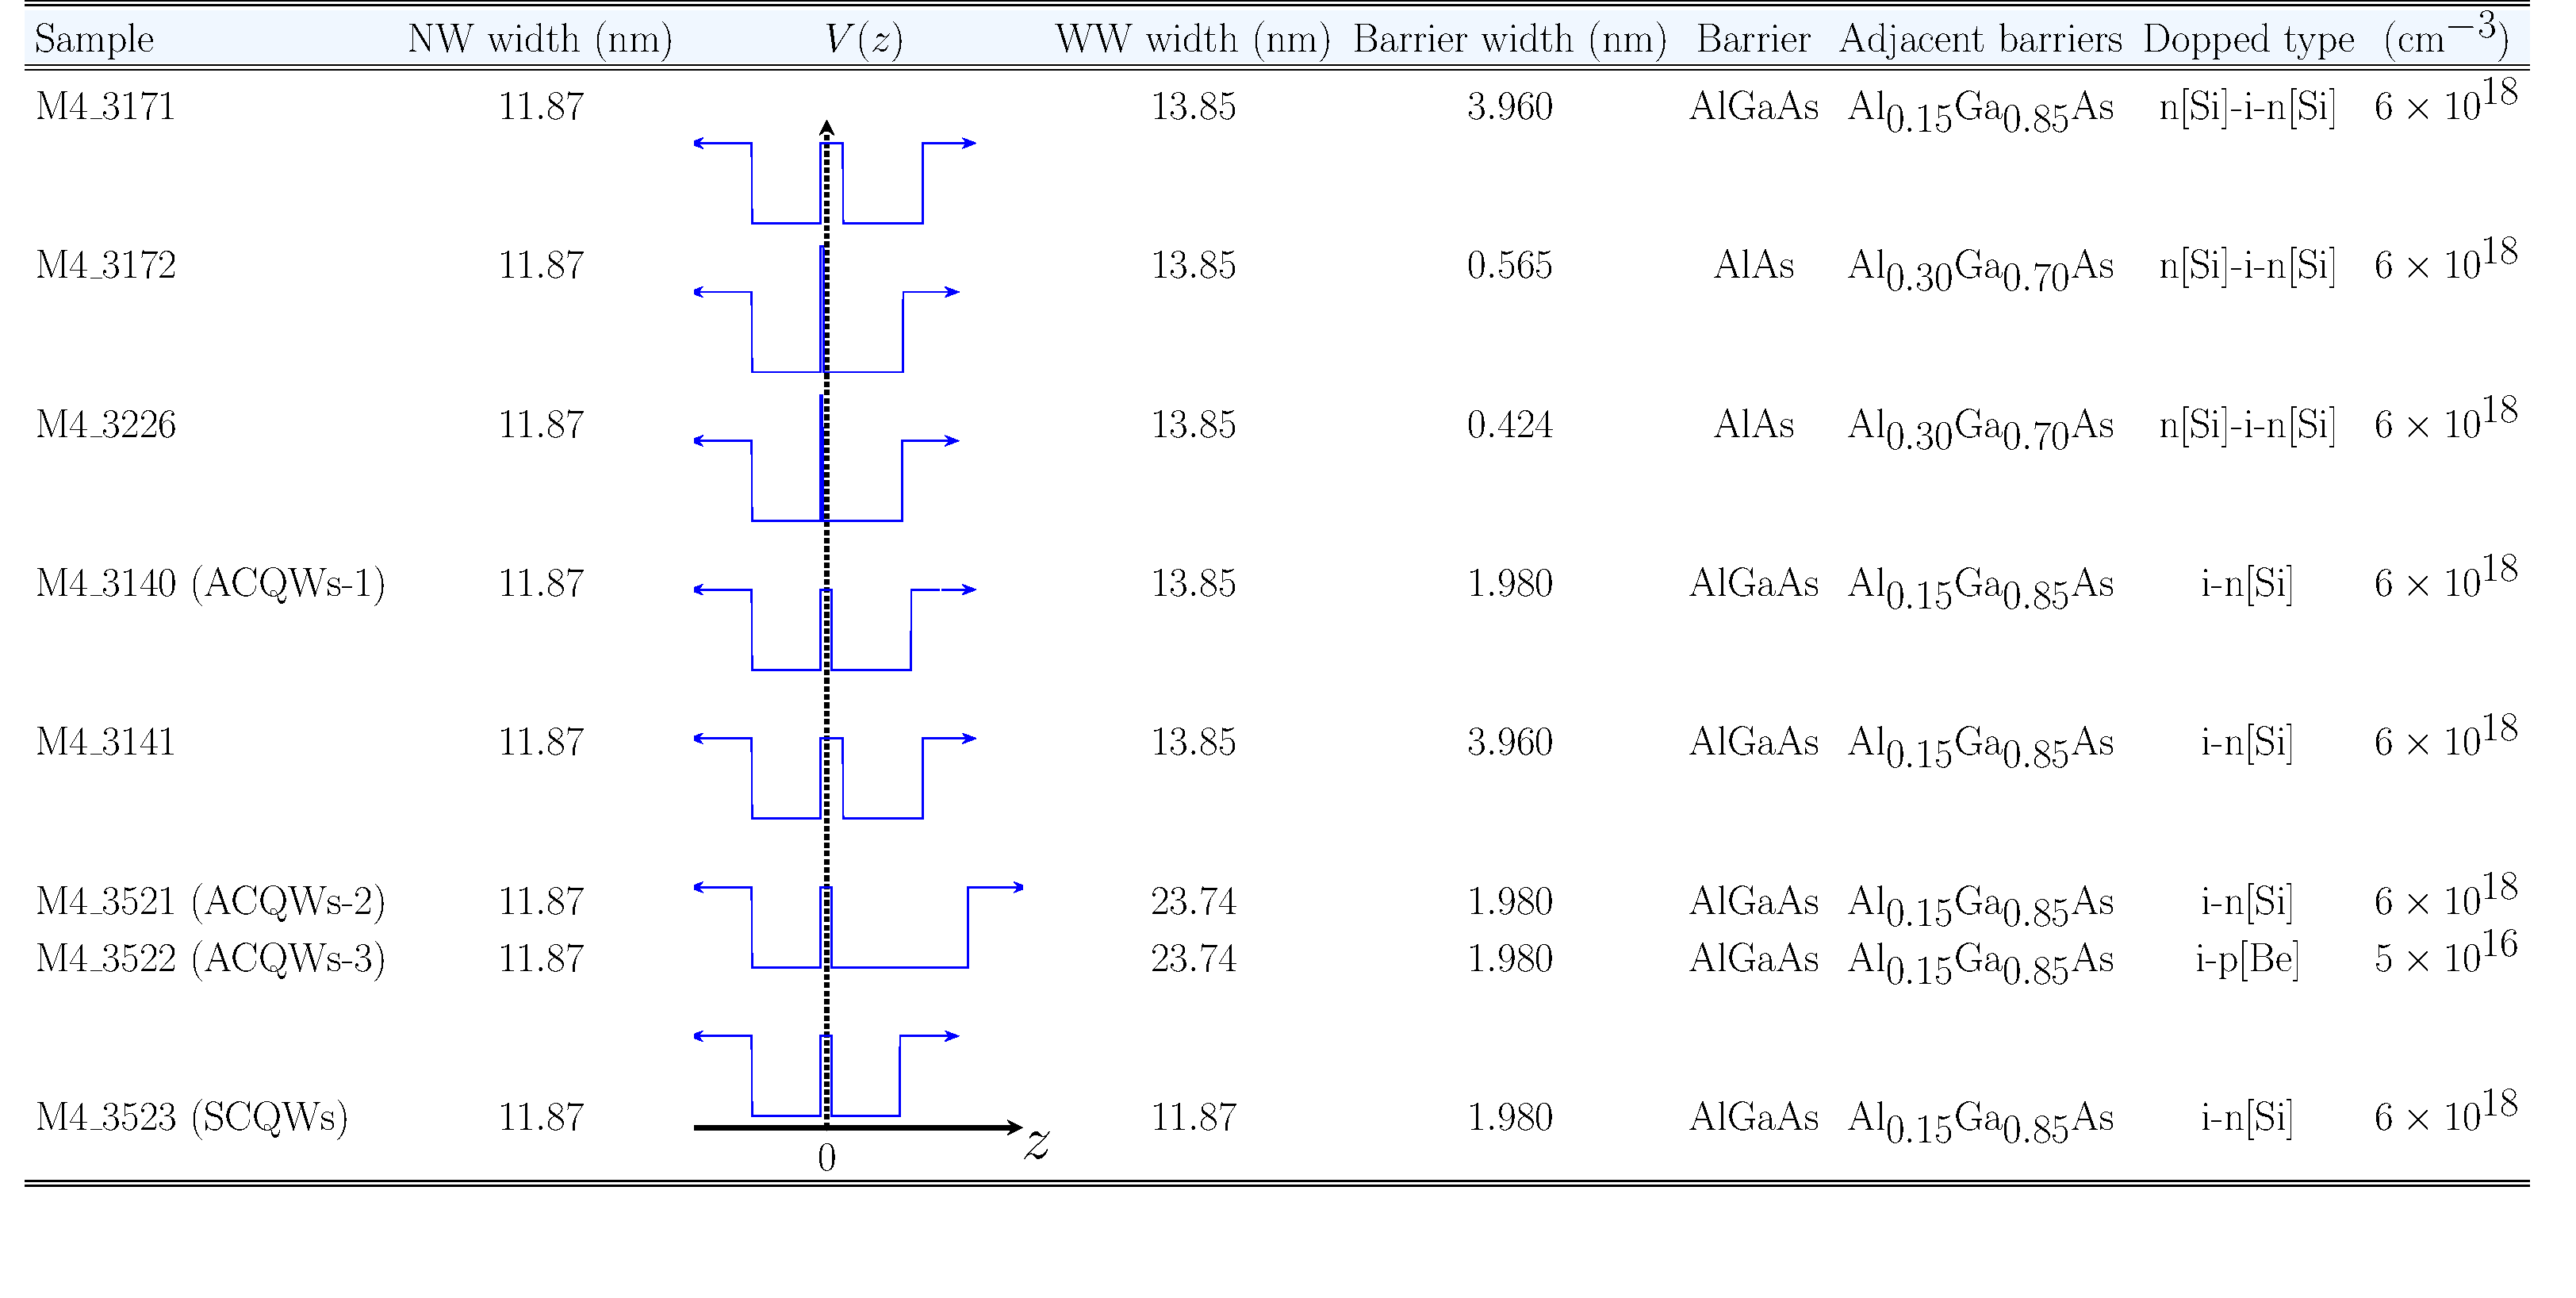
\includegraphics[width=\textwidth]{../tables/chapter-3/table-1-samples/build-ruco/table-1-samples.pdf}
		\caption[Table of samples description]{This table shows the CQWs structures studied in this work.  CQWs potential profiles $V(z)$ are shown to observe the different shapes, composition parameters, and dimensions of structures studied. The dashed line determines the symmetric reference in the last samples in which we focused (\tucu, \tcvu, \tcvd, \tcvt), due to their characteristic results. }
		\label{tab:chapter3:Samples description} 
	\end{table}
\end{landscape}
%  Worth mentioning that the purpose of the first four samples (up to down in table) they were grown with the objective of measure indirect excitons (IX), so that,  the structures are more complex, and we omitted the value of n-doped since these samples are doping in bottom and top to minimize the intrinsic electric field (screening field effect) so that external perturbation is applied through a voltage over the sample\cite{yuan2018tunneling} and the n-doped enhance the external perturbation \footnote{Non-published, the specific information about the doped  in these growths, if you have a question about this, you can send email to Dr. Klaus Biermann \url{biermann@pdi-berlin.de}}. 

After realized experiments over the four first samples and observe possible trions  (\xp or \xm)  through \gls{PR} spectroscopy and an apparent increase of the RAS signal, it was decided to focus the experiments on these structures, which have a less complex composition as in the case of the first three samples in the table (see \Cref{tab:chapter3:Samples description}). Therefore,  it took the sample \tucu as a  basis, i.e., same barriers widths both coupling barrier and adjacent barriers, obtained the samples \tcvu, \tcvd and \tcvt where sample \tcvd is the same to sample \tcvu in structure but with a different type of doping (p-type in \tcvd and n-type in \tcvu), samples \tcvu and \tcvd have the same doping type (n-type in both) but one of the QW is more width to another, this means that the sample \tcvt have the same thickness in both QWs (SCQWs) and sample \tcvu have one  QW  thick more than the another (ACQWs). 

The \Cref{sec:chapter 3 Spectroscopy}  shows each experimental setup implemented in this investigation with their respective results. Starting with the  \Cref{subsec:chapter-3-pl} shows PL spectroscopy, their experimental setup implemented to obtain transitions energies values and compare with numerical results, after,  in \Cref{subsec:chapter-3-pr} shown experimental setup and results of the PR spectroscopy, to get information about the intrinsic electric field and the effects caused by this. Finally,  \Cref{subsec:chapter-3-ras} shows the RAS experimental setup and exposes the experiments that were realized to study the anisotropy caused by the asymmetry due to the relative thickness between the CQWs.

\section{Spectroscopy: Experimental Setups and Results}
\label{sec:chapter 3 Spectroscopy}
\vspace{-10mm} 
\lettrine[lines=3, lraise=.1, nindent=0mm, slope=0mm]{\textbf{O}}{ptical spectroscopy} frequently is defined as a branch of physics that studies the \emph{light-matter interaction}, this is important because the simple definition of interaction covers a vast realm of physical phenomena from classical to quantum electrodynamics\cite{weiner2017light}. Therefore, optical spectroscopy is an essential tool in experimental solid state physics, gives the guide to study optical and electronic properties of semiconductors.\\*
The optical process in semiconductors consists of the study of response due to \emph{light-matter interaction}, this response corresponds basically to the processes that can occur in the solids when light\footnote{Refers to light due to radiation spectral range} falls on (photons) in it. These processes are absorption, reflectance, emission, and scatter where all of this depends on electromagnetic spectra range, in our case this range includes from near-infrared to mid-infrared (700nm to 900nm).  Although those processes are of the utmost importance, optical spectroscopies that uses in this work involve more interest in absorption and emission, being the latter sensed in our experimental setups.  \\

\begin{figure}[H]
	\centering
	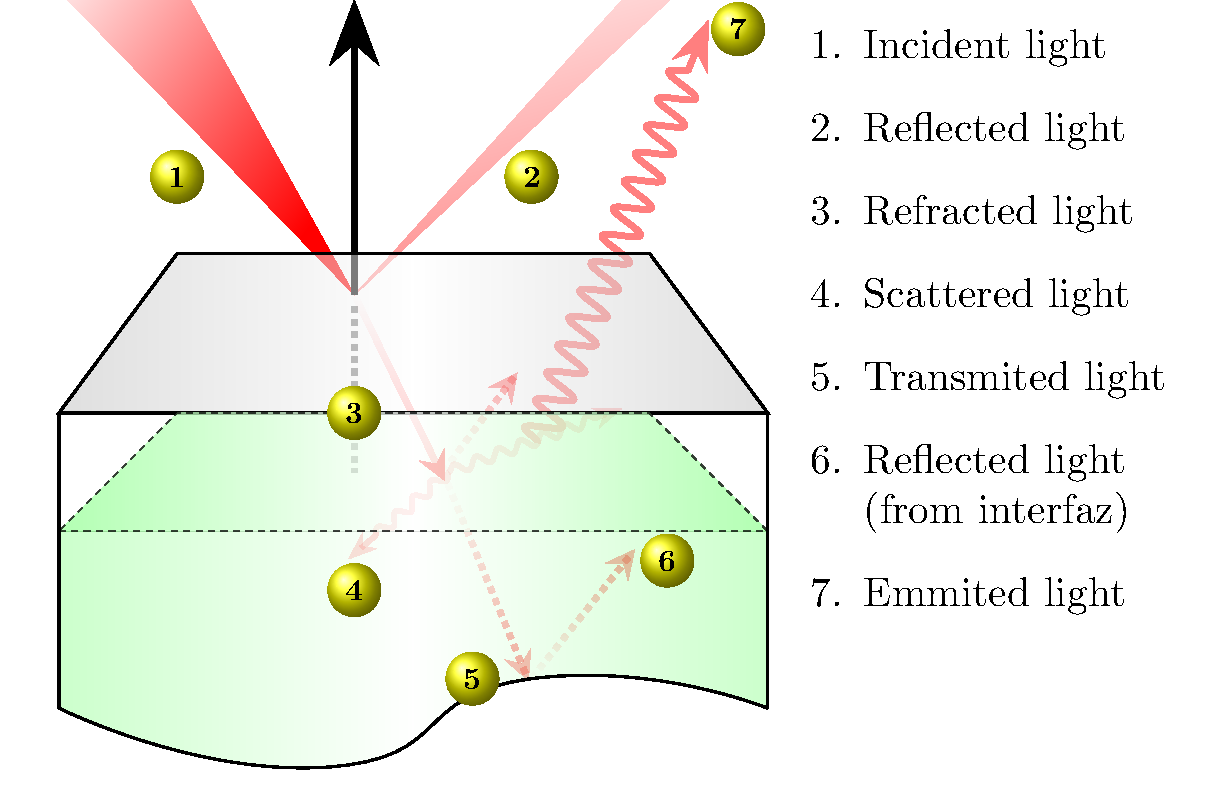
\includegraphics[width=0.8\textwidth]{../figures/chapter-3/lmi-process/build/lmi-process}
	\caption{Processes that occur inside a solid in the light-matter interaction phenomena.}
	\label[figure]{fig:Section-3.1-light-matter-interaction}
\end{figure}


Before continuing with the manuscript of this chapter, I would like to mention that the experiments could not be carried out without the development of detectors, specifically optical detectors. To speak about optical detectors, it is impossible not to mention the photoelectric effect that in general terms is the transfer of energy from photons to electrons when the light spot on a surface\cite{einstein1905uber}. So, this fundamental quantum phenomenon is the basis of detectors in spectroscopy, these detectors are called photodetectors, where these convert the light power(photons incidence over their sense area)  into an electric signal, voltage, or current, then this signal we can measure and amplify it. The next sections will mention and discuss the PD implemented in the experimental setup and especially which are the pros and cons. It is important that the photo-cathode of the photo-detector corresponds to the spectral range of experiments. i.e, in our experiments the spectral range of interest is from 700nm to 900nm the PD should have characteristics to adequate of this range. The \Cref{tab:chapter-3-section-samples-photodectors-materials} shows some PD and their characteristics\cite{tkachenko2006opticalspectroscopy}. 
\begin{table}
	\centering
	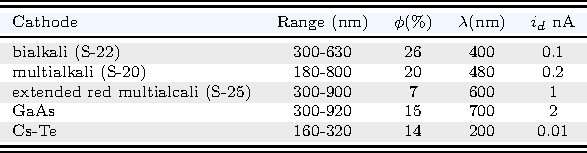
\includegraphics[width=\textwidth]{../tables/chapter-3/table-photodetectors/out/photodetectors.pdf}
	\caption{Photo-cathodes,usually implemented in PD to the spectroscopy of semiconductors\cite{tkachenko2006opticalspectroscopy}. }
	\label{tab:chapter-3-section-samples-photodectors-materials}
\end{table}

% \newcolumntype{C}{>{\centering\arraybackslash}p{22mm}}% a centered fixed-width-column
% \begin{table}[H]
% 	\centering
% 	\begin{tabular}{lCCCC}
% 		\hline
% 		\hline
% 		cathode &  range (nm) &  $\phi$ (\%) & $\lambda_{m}$ (nm) & $i_{d}$ nA\\
% 		\hline
% 		 bialkali (S-22) &  300-630 & 26 & 400 & 0.1\\
% 		 multialkali (S-20) & 180-800 & 20 & 480 & 0.2\\
% 		 extended red multialcali (S-25) & 300-900 & 7 & 600& 1\\
% 		 GaAs & 300-920 & 15& 700 &2\\
% 		 Cs-Te & 160-320 & 14 & 200 & 0.01\\
% 		\hline
% 		\hline
% 	\end{tabular}
% \caption{Photo-cathodes,  usually implemented in PD to the spectroscopy of semiconductors\cite{tkachenko2006opticalspectroscopy}.}
% \label{tab:chapter-3-section-samples-photodectors-materials}
% \end{table}

As a comment, it is important to denote that the CCD devices are being span in many setups in recent years and this is because these devices enlarged the range of experiments that can be realized with these, above all in other areas of physics as in the experimental astrophysics in which has obtained awfully important results.  Nowadays, CCD devices in experimental solid-state physics have contributed to getting great experiments that previously were limited due to spatial resolution and time response.  In the \cref{subsec:chapter-3-pl}, it discusses the advantages and cons of the detectors (PD and CCD)  in PL spectroscopy context. 


\subsection{Photoluminiscence Spectroscopy (PL)}
\label{subsec:chapter-3-pl}
\vspace{-10mm}
\lettrine[lines=3, lraise=.1, nindent=0mm, slope=0mm]{\textbf{P}}{hotolumniscense} spectroscopy is characterized by be a fast spectroscopy to get optical properties (\textit{i.e.} band-gap) and transitions in  semiconductor materials, for this reason the work began with PL spectroscopy with aim of searching optical transitions in each CQWs samples and compare with  numerical solution of one-dimensional Schr\"{o}dinger equation (see \Cref{tab:sec-chapter-2-numerical-results}). 
\begin{figure}
	\centering
	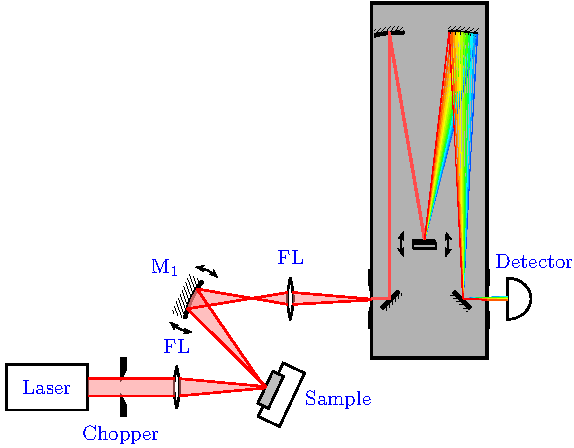
\includegraphics[width=\textwidth]{../figures/chapter-3/pl-setup/build-ruco/pl-setup}
	\caption[PL Scheme]{Scheme of photoluminiscense setup allowing measurements at 14 K, a laser with wavelength of 685nm anda Si detector in tandem were used.}
	\label{fig:chapter-3 subsec 3.2.1 PL setup}
\end{figure}
 
Although PL signal is characterized by be greater than other spectroscopies implemented in this work, the need to use a chopper is only to filter the signal to the external noise, this is achieved used a lock-in amplifier where the reference signal is the chopper and signal input is first measured by a multimeter and then input in the lock-in amplifier. In many other experimental setups the experimental measure are take  fast,  this is because  implement a CCD device as a detector of experimental signals, where  these devices are distinguished by fast time of acquisition (apart from other reasons). In our case the time of measure it does not comparable with those, due the time in our experiments is about 2 hours (explained latter) and those are about several minutes. But why use lock-in amplifier if CCD devices shorter measured time?\\
The answer is not be for impatients\footnote{The author self-considers impatient}, the reason is that, the lock-in and detector implementation allow control over spectral resolution through two parameters, the first one is in the choice of monochromator's slits apertures and the second one has to do with step wavelength this is the  progress step by step over the spectral range taking into account in the experimental measure. Also, the step by step experiments provide the choice of measures  number in each step where finally only consider the average of these points, resulting more clean spectra in compare with CCD setups\footnote{Even if modify time and average of measures, the spectra measured with lock-in amplifier are more quality.}. Although the time is important  worth it inverts  to  get quality experiments. 

Some experiments shown below correspond to Carlos's bachelor thesis \cite{carlos2020thesis}, who implemented a simple and reliable PL system also he makes a computational code to fit PL spectra using numerical and experimental results (you can check Carlos's codes in our laboratory  repository on GitHub\footnote{\url{https://github.com/NanophotonIICOs}}). These results were correlated with previously   realized  experiments taking into account the same parameters. 


The experiments are organized by labels, how shows in \Cref{tab:chapter3:Samples description}, started with the samples \m{1}{7}{1}, \m{1}{7}{2} and \m{2}{2}{6} where these samples were grown with objective the measure trions. The experimental parameters are shown in \Cref{tab:CH 3 PL experimental parameters}, in each experiment the optical setup was optimized to enhance the signal measured, the optimization process consisted in measure laser peak at a definite monochromator slits aperture then finely move the mirror until achieving a high response in multimeter, repeat this closing the slits and measuring the FWHM of the laser peak in each step, finally we obtained an optimal resolution about 1 nm in our \gls{PL} experiments. 

% \begin{table}[t]
% 	\centering
% 	\pgfplotstableread[col sep=comma]{
% 		sample,laser,range,step,lectures,slits
% 		\m{1}{7}{1},680,800-820,0.1,20,75
% 		\m{1}{7}{2},680,780-840,0.1,15,75
% 		\m{2}{2}{6},680,800-820,0.1,20,100
% 		\m{1}{4}{0},680,800-820,0.1,20,100
% 		\m{1}{4}{1},680,800-820,0.1,20,100
% 		\m{5}{2}{1},680,800-820,0.1,20,100
% 		\m{5}{2}{2},680,800-820,0.1,20,100
% 		\m{5}{2}{6},680,800-820,0.1,20,100
% 	}\pltable
% 	\pgfplotstabletypeset[%
% 	%Draw rules
% 	every head row/.style={before row=\toprule\toprule\rowcolor{aliceblue},after row=\midrule},
% 	every last row/.style={after row=\bottomrule\bottomrule},
% 	every even row/.style={
% 		before row={\rowcolor[gray]{0.92}}},
% 	%Column styles
% 	columns={sample,laser,range,step,lectures,slits},
% 	columns/sample/.style={string type,column name=Sample, column type=c}, 
% 	columns/laser/.style={string type,column name=Laser, column type=c}, 
% 	columns/range/.style={string type, column name=Range(nm), column type=c}, 
% 	columns/step/.style={ string type, column name= $\lambda$ step (nm),column type=c}, 
% 	columns/lectures/.style={string type, column name=No. of singnal acquisition,column type=c}, 
% 	columns/slits/.style={numeric type,column name=Slits apereture ($\mu$m),column type=c}, 
% 	]{\pltable}
% 	\caption{PL experimental parameters implemented in each sample, all experiments were carried about 14K and was used the same red (680 nm) laser diode.   The measured parameters as a Wavelength step or number of acquisitions per step Wavelength were optimized as explains in the text.  }
% 	\label{tab:CH 3 PL experimental parameters}
% \end{table}


\begin{table}[H]
	\centering
	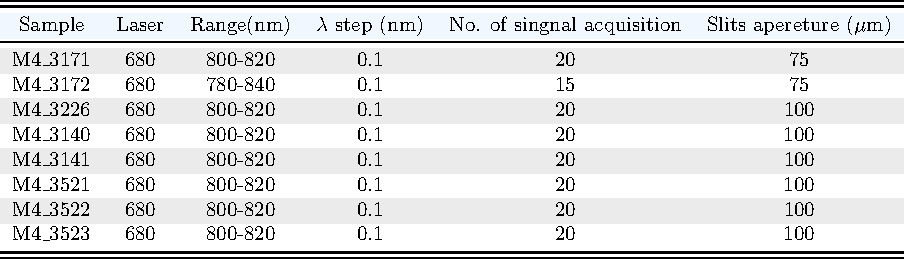
\includegraphics[width=\textwidth]{../tables/chapter-3/table-pl-parameters/out/pl-parameters.pdf}
	\caption[Table of PL experimental parameters]{PL experimental parameters implemented in each sample, all experiments were carried about 14K and was used the same red (680 nm) laser diode.   The measured parameters as a Wavelength step or number of acquisitions per step Wavelength were optimized as explains in the text.  }
	\label{tab:CH 3 PL experimental parameters}
\end{table}

\begin{figure}[hbt!]
	\centering
	\begin{subfigure}{\textwidth}
		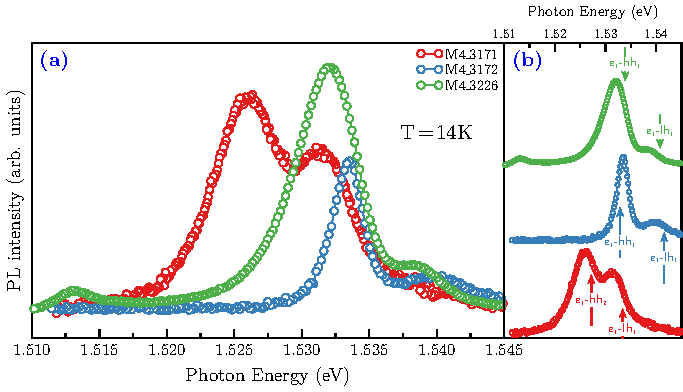
\includegraphics[width=\textwidth]{../figures/chapter-3/pl-plots/build-ruco/pl-1}
		\phantomsubcaption\label{subfig:chapter-3-PL-experiments-M4_3171-M4_3172-M4_3226-a)}
		\phantomsubcaption\label{subfig:chapter-3-PL-experiments-M4_3171-M4_3172-M4_3226-b)}
	\end{subfigure}
	\caption{ 
		%Subfigure \subref{subfig:chapter-3-PL-experiments-M4_3171-M4_3172-M4_3226-a)} shows PL experiments of the samples \m{1}{7}{1}, \m{1}{7}{2} and \m{2}{2}{6}, where show spectra and results measured at 14K. Plots in how the comparison between these samples, where clearly can see the relative intensity among in each experiment. In \subref{subfig:chapter-3-PL-experiments-M4_3171-M4_3172-M4_3226-b)} it can be seen each PL spectra with the  respective direct transitions numerically calculated, hh1 and lh1 indicates  the first energy level that corresponds to heavy- and light-holes respectively.
\subref{subfig:chapter-3-PL-experiments-M4_3171-M4_3172-M4_3226-a)} shows PL experiments of the samples \m{1}{7}{1}, \m{1}{7}{2} and \m{2}{2}{6} at 14K. Plots in how the comparison between
these samples, where clearly can see the relative intensity among in each experiment. In \subref{subfig:chapter-3-PL-experiments-M4_3171-M4_3172-M4_3226-b)} it
can be seen each PL spectra with the respective direct transitions, numerically calculated, $\mathrm{hh}_1$
and  $\mathrm{lh}_1$ indicates the first energy level that corresponds to heavy- and light-holes respectively.}
		\label{fig:chapter-3-PL-experiments-M4_3171-M4_3172-M4_3226}
\end{figure}



An important detail about module laser ThorLabs and very remarkable in the \Cref{subsec:chapter-3-pr} is related to power, the power of this was not stable in some time periods causing a variation in the results, this is the reason to use different experimental parameters  and after some test were optimized the choice  of the Wavelength step, number of acquisitions per $\lambda$ step and slits aperture, this depending on each sample. 

The PL spectra, corresponding to the samples showing in \Cref{subfig:chapter-3-PL-experiments-M4_3171-M4_3172-M4_3226-a),subfig:chapter-3-PL-experiments-M4_3171-M4_3172-M4_3226-b)},  were more complicated to interpret and in experimental conditions as well. For this reason, we decided to calculate the absorption along of the structure that composes each sample because due to they have more layers. We speculated that this is the reason as to why it is  complex to realize the experiments and their analysis. As previously spoken, the study of light-matter interaction in solids can be a headache this is because in real experiments more than one interaction mechanism can be observed, especially in PL spectroscopy and, the objective is to measure only one of them, therefore, the experimental results can be affected and complicate their interpretation. The reason for starting with the samples of \Cref{fig:chapter-3-PL-experiments-M4_3171-M4_3172-M4_3226} is that they have effects that modify the PL spectra and, although these effects are very interested in our case, they reduce the PL signal.\\* 


If started with the scoop, that the PL spectrum in semiconductors is given by an interband emission generated by recombination carriers, and this, in turn, is due to the absorption of photons provided by an excitation laser source. Therefore, the PL signal is due to absorption, it does not matter that they are opposite processes, the absorption, as well as many other mechanisms of light through the solid, can modify and generate the spectrum of PL. The absorption analysis was carried on in the macroscopic approach to light-matter interaction (in \Cref{chap:Intro}, talks about quantum processes and aspects of light-matter interaction in a microscopic environment), therefore,   can use classical electrodynamics to study optical properties of semiconductors. One crucial property of semiconductors is the dielectric function, this is proportional to the complex refractive index (later it is named only as refractive index) and with this,  can be described the optical properties of semiconductors. It is important to mention that the refractive index describes how light propagates  in a medium, and it expressed as\cite{chuang1995physics,jimenez2016spectroscopic}:

\begin{equation}
	\tilde{n}=n + i\kappa = \sqrt{\epsilon(\omega)},
	\label{eq:chapter-3-PL-complex-refractive-index}
\end{equation}

where the real part ($n$) represents the refractive index and the imaginary part ($\kappa$) is the extinction coefficient.  Even if the objective of this work does not rewrite and reinterpret the physics of these phenomena, we will try to focus on specific equations to reach the goal, which is the absorption model in semiconductors. Then the electric field inside a solid can be written as\cite{jimenez2016spectroscopic,lu2018spectroscopy,ball2001basicsspectroscopy}:  

\begin{equation}
	\mathbf{E} = \mathbf{E_0}\exp\left({\dfrac{-\kappa\omega  z}{c}}\right) \exp\left({-i\omega\left( \dfrac{nz}{c}-t\right)}\right).
    \label{eq:chapter-3-PL-electric-field-in-solid}
\end{equation}

 In \Cref{eq:chapter-3-PL-electric-field-in-solid}, can see the solution of Maxwell equation in a macroscopic picture of the photon-material interactions. This represents a wave propagating with dispersion and staying in terms of refractive index, but the principal idea is to establish a relationship that can help us to describe the absorption in terms of these principal parameters. The absorption is a process that occurs in any spectroscopy and is the absorption coefficient that defines such a feature in each medium. The extinction coefficient $\kappa$ is the cause of the wave damping when the electromagnetic wave crosses in media, therefore it is related by absorption coefficient. Now in \Cref{fig:Section-3.1-light-matter-interaction} can see that there are three principal parts, that they are intensities that are reflected, transmitted, and absorbed. These three parts compose the original incident light through:
 
\begin{equation}
	\mathrm{I_0}=\mathrm{I_R}+\mathrm{I_T}+\mathrm{I_A}.
	\label{eq:chapter-3-Intensities-of-light}
\end{equation}


Finally, we call upon one of the most notable laws in spectroscopy, this basic  expression relates the intensity of light absorbed with the absorption coefficient and is known as Beer-Lambert law\cite{demtreder2019electrodynamics,sole2005introductionspectroscopy}: 

\begin{equation}
	\mathrm{I}(z) = \mathrm{I_0}\cdot e^{-\alpha z},
	\label{eq:chapter-3-Beer-Lambert-Law}
\end{equation}

then this tell us how intensity decrease as a function of absorption coefficient.  As a result of these basic principles in a real structure, we can define de absorption in each layer. After these general and quick basics of the macroscopic basis of light-matter interaction, let's move to a more realistic environment where the calculations are more complex and where it is decided that parameters have major physical priority. The numerical solutions of absorption along structure were carried out using an exceptional Open-Source code called \textbf{SOLCORE}\cite{alonso2018solcore}\footnote{You can test and contribute this code, visiting their GitHub repository at \url{https://github.com/qpv-research-group/solcore5.git}. } and our codes. As previously mentioned in a real calculation is frequently taken into account only parameters with major physical sense depending on the situation, arduous computational solutions, or for simplicity. From \textbf{SOLCORE}, we have the simplest model to calculate the absorption, despising all reflections at the interfaces having only the absorption as a function of wavelength and depth $z$ expressed as: 


\begin{equation}
	A_{n}(\lambda,z) = \alpha_{n}(\lambda)\exp\left(-\sum\limits_{i=1}^{n-1}\alpha_{i}\left(\lambda\right)d_i-\alpha_{n}\left(\lambda\right)\left(z-z_{n}\right)\right),
	\label{eq:chapter-3-SOLCORE-Absorption}
\end{equation}

where $\alpha_{n}$ is the absorption of layer $n$, $d_{i}$ is the thickness and $z_{n}$ the position of beginning of the layer\footnote{In \cref{eq:chapter-3-SOLCORE-Absorption} originally the thickness is represented how $w_i$, by confusion issues it was decided to change the notation.   }. 

\begin{figure}[hbt!]
	\centering
	\begin{subfigure}{\textwidth}
		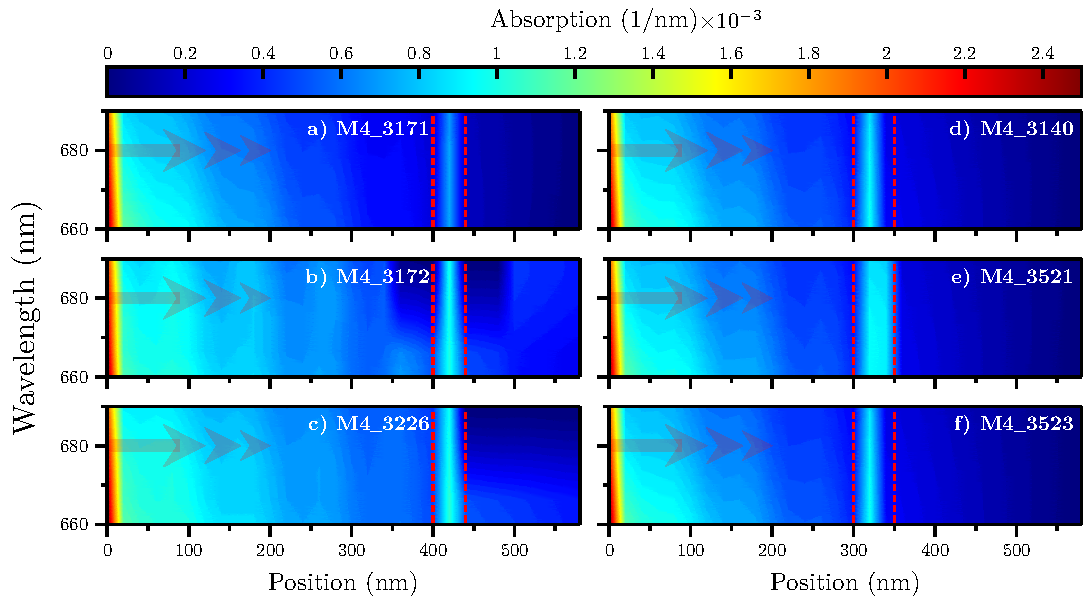
\includegraphics[width=\textwidth]{../figures/chapter-3/absorption-simulations/build/abs-calcs.pdf}
		\phantomsubcaption\label{subfig:chapter-3-Absorption-M4_3171-a)}
		\phantomsubcaption\label{subfig:chapter-3-Absorption-M4_3172-b)}
		\phantomsubcaption\label{subfig:chapter-3-Absorption-M4_3226-c)}
		\phantomsubcaption\label{subfig:chapter-3-Absorption-M4_3140-d)}
		\phantomsubcaption\label{subfig:chapter-3-Absorption-M4_3521-e)}
		\phantomsubcaption\label{subfig:chapter-3-Absorption-M4_3523-f)}
	\end{subfigure}
	\caption{
		%Absorption calculated as a function of sample depth, dashed lines closed the CQWs region, left: \Cref{subfig:chapter-3-Absorption-M4_3171-a),subfig:chapter-3-Absorption-M4_3172-b),subfig:chapter-3-Absorption-M4_3226-c)},here the samples have \algaas layers with different compositions $x=0.15$,$x=0.2$ and $x=0.3$ this results in a change of refractive index then also expected in absorption.  Right: \Cref{subfig:chapter-3-Absorption-M4_3140-d),subfig:chapter-3-Absorption-M4_3521-e),subfig:chapter-3-Absorption-M4_3523-f)} these samples are equal in structure but change the width of one oM4a)f the QWs, therefore the absorption manifests more homogenous than the first three samples. 
Absorption calculated as a function of sample depth. Dashed lines closed the CQWs
region, left: \Cref{subfig:chapter-3-Absorption-M4_3171-a),subfig:chapter-3-Absorption-M4_3172-b),subfig:chapter-3-Absorption-M4_3226-c)}. Here the samples have \algaas layers with different compositions $x = 0.15$, $x = 0.2$ and $x = 0.3$; this results in a change of refractive index then also in the absorption. Right: \Cref{subfig:chapter-3-Absorption-M4_3140-d),subfig:chapter-3-Absorption-M4_3521-e),subfig:chapter-3-Absorption-M4_3523-f)}these samples are equal in structure but different on their width of one of the QWs, therefore the absorption manifests strongly homogenous than the first three samples.
	}
	\label{fig:chapter-3-PL-Absorption-Calcs}
\end{figure}

The samples with extra layers have characteristics that do not present in samples with fewer layers, one of this is which the fundamental transition around the GaAs gap does not possible to observe in these samples, the amplitude in these samples in comparison with sample \sm{3141} for example, is around of twenty times smaller than this, opposite case in samples \sm{3140}, \sm{3421}, \sm{3523}. We take these samples because these are the basis of this work, the complete set of PL experiments corresponds to the work previously mentioned. So, why is the important to get the PL results and calculate absorption?
The answers are simple, the importance to get PL spectra to help us to get experimentally energy transitions, which have a very important role in the next experiments and in the basis of our model to explain the increase in anisotropy in the ACQWs.  Also, the experimental PL results are the basis to compare that our numerical calculations are consistent with the experiments. Numerical calculations get more complicated in bigger structures, this means, while the structure is conformed with more layers and these layers are thicker, the probability to get a divergence in calculations is great, this is the reason which not all models work. In fact, in our numerical calculations the energy transitions in samples with more layers (\sm{3171}, \sm{3172}, \sm{3226}) we had to be careful at the moment to choice energy binding, the reasons are many and in the PL is complicated to get unique information and even less in structures with high doped, the charge recombination they play us dirty to understand the results. \\*
The case of absorption calculations is a guide to explain the difficulty to carried out PL experiments and put to discussion if doping is a reason to generate or not intrinsic electric field, after all the absorption is part of field solutions. 

\Cref{subfig:chapter-3-Absorption-M4_3171-a),subfig:chapter-3-Absorption-M4_3172-b),subfig:chapter-3-Absorption-M4_3226-c)} are the calculations of absorptions as a function of depth, where previously explained, it was only taken into account classical regime therefore the absorption remains in terms of the optical parameters of each layer which conforms all structure. In these figures can shows that in a range of 650 nm to 700 nm the wavelengths are absorbed with major proportion in the first layer, this is due to the structures starts with a GaAs doped(n- or p-type) or undoped layer. After along in structures, also can observe the  decrease absorption to short wavelengths, and the notably increased around of the coupled quantum wells.


\begin{figure}[H]
	\centering
	\begin{subfigure}{\textwidth}
		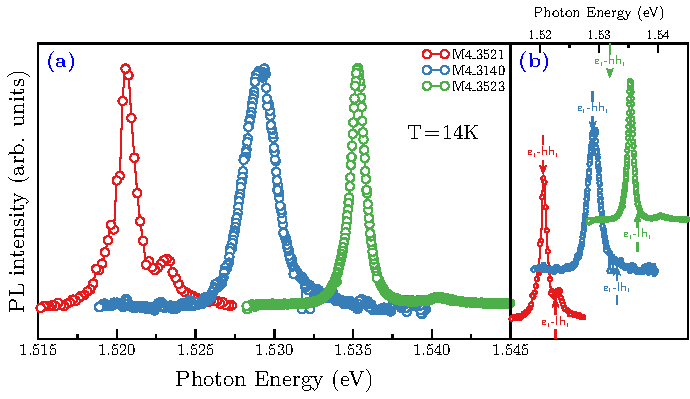
\includegraphics[width=\textwidth]{../figures/chapter-3/pl-plots/build-ruco/pl-2}
		\phantomsubcaption\label{subfig:chapter-3-PL-experiments-M4_3140-M4_3521-M4_3523-a)}
		\phantomsubcaption\label{subfig:chapter-3-PL-experiments-M4_3140-M4_3521-M4_3523-b)}
	\end{subfigure}
	\caption{\subref{subfig:chapter-3-PL-experiments-M4_3140-M4_3521-M4_3523-a)} Shows the PL spectra of samples \sm{3140}, \sm{3521} and \sm{3523}, in this comparison is clear the shift  between these in respect to first transitions. The relative change in width of one of the QW modifies the  energy transitions being the sample 3521 the lowest energy. \subref{subfig:chapter-3-PL-experiments-M4_3140-M4_3521-M4_3523-b)} It is plotted  each PL spectra result with the correspondent $\thh{1}{1}$ and $\tlh{1}{1}$ transitions energies. }
	\label{fig:chapter-3-PL-experiments-M4_3140-M4_3521-M4_3523}
\end{figure}

These calculations make sense in the next section where PR spectroscopy is a powerful tool that can used to measure the optical properties due to the modulation without external perturbation, this means that the modulation depends on the intrinsic properties of the structure. The generalizability of the results is limited by the classical regime, as previously mentioned, it has taken into account the refractive index where the absorption can obtain from the complex part of this,  that is the extinction coefficient. The common use of the PL is to determine the band gap and optical transitions in semiconductors, especially in QS as quantum wells, but what happens if consider PL regardless of the penetration depth? 
In our case it is important does not, due to the structures studied have wide layers before of coupled quantum wells region, this can observe in figure 4 where shows the results of samples: \sm{3171}, \sm{3172}, \sm{3226}, \sm{3140}, \sm{3521}, and \sm{3523}.  In the PL experiments carried out here,  it was used as a show in \Cref{fig:chapter-3 subsec 3.2.1 PL setup} a red laser diode 
of  $\lambda=$685 nm, although the laser energy is chosen in respect to energy gap therefore short wavelengths are preferable but how we can see these wavelengths are absorbed in the first layer due to the samples ends in a GaAs layer, even the laser used is absorbed in large proportion. 

Contrary to the samples measured first, the samples \sm{3140}, \sm{3521}, and \sm{3526} exhibits the most spectral resolution this means that exhibit a more homogenous behavior  due to the QWs have quantized energy, therefore, the electron-hole recombination is more probably to measure than the other samples which present width spectrums so that these results may be due to the several internal mechanisms of which can be: impurities, large carrier density due doped,  defects, among others\cite{khmissi2010effectcarriers,kundrotas2005excitonic}. In each of these PL spectra, \Cref{fig:chapter-3-PL-experiments-M4_3171-M4_3172-M4_3226,fig:chapter-3-PL-experiments-M4_3140-M4_3521-M4_3523} present the most intense peaks associates with heavy- and light-holes exciton transitions denoted by $\thh{1}{1}$ and$\tlh{1}{1}$ respectively.


\begin{table}[H]
	\centering
	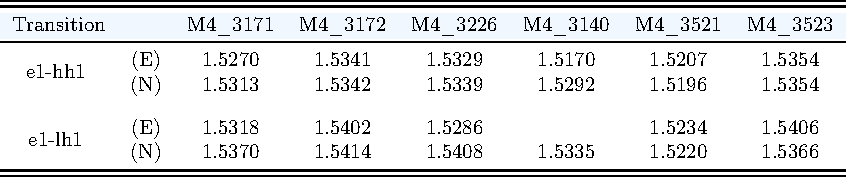
\includegraphics[width=\textwidth]{../tables/chapter-3/pl-comparison-numerical/out/pl-comparison-numerical.pdf}
	\caption{Comparison table between experimental transitions obtained trough PL measures and numerical transitions calculated as explained in \Cref{sec:chapter-2-numerical-calculations}}
	\label{tab:CH-3-PL-Experimental-vs-Numerical-transitions}
	% \pgfplotstableread[col sep=&, row sep=\\]{
	% transition&T&m43171   &m43172   &m43226   &m43140   &m43521   &m43523\\
	% e1-hh1    &(E)&1.5270   &1.5341   &1.5329   &1.5170   &1.5207   &1.5354\\
	%           &(N)&1.5313   &1.5342   &1.5339   &1.5292   &1.5196   &1.5354\\
	% e1-lh1    &(E)&1.5318   &1.5402   &1.5286   &         &1.5234   &1.5406\\
	% 		  &(N)&1.5370   &1.5414   &1.5408   &1.5335   &1.5220   &1.5366\\
	% }\energy
	% 	\pgfplotstabletypeset[%
	% 	CellColor/.style={postproc cell content/.append code={
	% 			\pgfplotstablegetelem{\pgfplotstablerow}{Color}\of{\mytable}%
	% 			\ifthenelse{\pgfplotsretval = 1 }% if 
	% 			{\pgfkeysalso{/pgfplots/table/@cell content/.add={\cellcolor{red}}{}}}% then
	% 			{}% else
	% 	}},
	% 	%Draw rules
	% 	every head row/.style={before row=\toprule\toprule\rowcolor{aliceblue},after row=\midrule},
	% 	every last row/.style={after row=\bottomrule\bottomrule},
	% 	columns/transition/.style={
	% 		assign cell content/.code={%
	% 			\pgfmathparse{int(Mod(\pgfplotstablerow,2))}%
	% 			\ifnum\pgfmathresult=0%
	% 			\pgfkeyssetvalue{/pgfplots/table/@cell content}%
	% 			{\multirow{2}{*}{##1}}%
	% 			\fi%
	% 		},
	% 	},
	% 	%every row 2 column 2/.style={postproc cell content/.append style={/pgfplots/table/@cell content/.add={\cellcolor{blue!10!white}}{},}},
	% 	%Column s
	% 	columns={transition,T,m43171,m43172,m43226,m43140,m43521,m43523},
	% 	columns/T/.style={string type,column name=\empty, column type=c}, 
	% 	columns/m43171/.style={column name=\sm{3171},fixed,fixed zerofill,precision=4,column type={c}},
	% 	columns/m43172/.style={column name=\sm{3172},fixed,fixed zerofill,precision=4,column type={c}},
	% 	columns/m43226/.style={column name=\sm{3226},fixed,fixed zerofill,precision=4,column type={c}},
	% 	columns/m43140/.style={column name=\sm{3140},fixed,fixed zerofill,precision=4,column type={c}},
	% 	columns/m43521/.style={column name=\sm{3521},fixed,fixed zerofill,precision=4,column type={c}},
	% 	columns/m43523/.style={column name=\sm{3523},fixed,fixed zerofill,precision=4,column type={c}},
	% 	]{\energy}
	\end{table}
	

In discussion with the before mentioned, several mechanisms can contribute to getting an inhomogeneous spectrum, even it can say that the two peaks which correspond to exciton transitions are thick and merge this can be related with the high doped level this is because very high dopant concentration causes an overlap of the impurity band with the free-carrier continuum\cite{kundrotas2005excitonic}. Table 5 shows the comparison between experimental transitions energies get with PL and the numerical results. It is important to mentioned that the approximation of numerical calculations are closed to experimental, the difference  is about of 5 meV for the PL case. It is well-known that the PL signal is increase as a function of decrease well widths, as shows 


\Cref{tab:CH-3-PL-Experimental-vs-Numerical-transitions} shows the comparison between experimental transitions energies get with PL and the numerical results. It is important to mention that the approximation of numerical calculations is closed to experimental, the difference is about 5 meV for the PL case. It is well-known that the PL signal is increased as a function of decrease well widths, this due to the energy of the confined particle state depends on strongly in it and this is demonstrated in \Cref{fig:chapter-3-PL-experiments-M4_3140-M4_3521-M4_3523} this due to structures does not have top n-type epitaxial layer these structures are i-n type, staying only barriers structures and PL line shape presents strong confinement \cite{singh1984theory,juang1986field,maluenda1983abrupttransitions}.



%++++++++++++++++++++++++++++++++++ PHOTOREFLECTANCE +++++++++++++++++++++
\addtocontents{toc}{\protect\newpage}
\subsection{Photorreflectance spectroscopy (PR)}
\label{subsec:chapter-3-pr}
\vspace{-10mm} 
\lettrine[lines=3, lraise=.1, nindent=0mm, slope=0mm]{\textbf{P}}{otoreflectance} belongs to the group of modulation spectroscopy, being one of the most important to determines field effects without external perturbations, this means that there is no need for an external source that generates the electric field on the sample. Exists another's kinds of modulation spectroscopy, where the type of modulation depends on interest effects, these can be phenomena linked with temperature (thermoreflectance), strain (piezoreflectance), electric (electroreflectance), etc. There is a great information amount of based on this technique, so it decides as previously mentioned and not to repeat in future chapters or sections, the principal idea is to focus on more representative expressions and phenomenological interpretation which be the best following our models and results. Unlike the PL the PR is the reflectance measure as a function of modulation or the changes in it, this once more needs to involve optical properties of the sample studied, in the \cref{eq:chapter-3-PL-complex-refractive-index} is expressed the refractive index with their real and imaginary part respectively and these are proportional to dielectric function. If the PR is the change in R which is due to modulation of an intrinsic electric field generated by doped layer o layers in the sample (later discuss this mechanism) this mean that:
\begin{equation}
	\dfrac{\Delta R}{R} = \dfrac{R_{\mathrm{off}}-R_{\mathrm{on}}}{R_{\mathrm{off}}},
	\label{eq:chapter-3-PR-mechanis}
\end{equation}


where $R_{\mathrm{off}}$ and $R_{\mathrm{on}}$ are the reflectivity when the perturbation (laser) are activate or not  are the reflectivity when the perturbation (laser) are activated or not, this mean that the results  falls on perturbation that is the laser.

The PR as modulation spectroscopy is a powerful tool to perform the study of semiconductors, their modulation mechanism occurs when the built-in field is screening by photoexcited carriers created through incident photons, which involves contactless and non-destructive.  In many cases, this spectroscopy technique is preferred due to it can measure transitions in heterostructures at room temperature in comparison with the PL or PLE\cite{shanabrook1987photoreflectance} that are measured at low temperature. Therefore, the highlighter characterize of the PR is the modulation of the built-in electric field, in part, this is due to the structure characteristics but in fact, the PR spectra is the change that generated electric field in the dielectric function, this is expected because is the result of measured the changes in reflectivity generated by the laser, in other words, the laser induces an excess of carriers which neutralize intrinsic field. This is well-known to study in the bulk materials, the models show as the reflectivity change is very well approximated by a first-derivative\cite{seraphin1972electric,aspnes1973surface,misiewicz1999photoreflectance,sydor1989photoreflectanceinterfaces}  but in QWs structures that are dominates by excitonic transitions then the PR line shapes can be understood in terms of modulation of dielectric function appropriate for excitons\cite{shanabrook1987photoreflectance,theis1988excitonic,theis1989extrinsic,gontijo1994photoreflectance}. 

\begin{figure}[ht!]
	\centering
	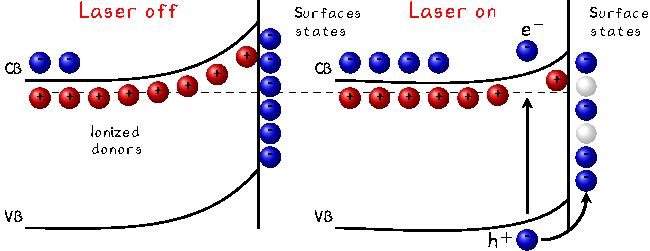
\includegraphics[width=\textwidth]{../figures/chapter-3/pr-modulation/build/pr-modulation.pdf}
	\caption{Scheme of the PR effect showing the carrier dynamics involved in the mechanism. Right and Left: the corresponding photoinduced changes when the laser is off and on, respectively. }
	\label{fig:chapter-3-PR-MODULATION-MECHANISM}
\end{figure}

Under the objective of this thesis, we have not focused on doing a traditional study of the line shape with their respective model, the study over PR lineshape is complex, the interpretation starting from changes in dielectric function like a derivative shape and depending on magnitude perturbation, i.e, does not is same the  PR analysis on structures with free carriers in solid that the confine particles in QWs structures, the bounded particles are not accelerated by built-in field modulation, so the energy spectrum is discrete and not continuous like free particles.  The capability to implement a lineshape fit,  renders PR be a great tool. 
It has been mentioned which the photoreflectance process is due to the built-in electric field modulation, therefore we are considering that the sample was grown considering desired characteristics to generate an intrinsic field, this means that sample contains n-type doped layers, impurities, unintentional strain mechanisms which generate a space charge region. In the case of an n-type doped layer in a structure, create a space charge region, this region creates the field therefore the conduction and valence bands are bending as a show in the \Cref{fig:chapter-3-PR-MODULATION-MECHANISM} and the Fermi energy are pinning at the surface. Photoexcited electron-hole pairs are separated by the built-in field, with the
minority carrier (holes in this case) being swept towards the surface.\\*
At the surface, the holes neutralize the trapped charge, reducing the built-in field\cite{misiewicz1999photoreflectance}. That is the general explanation to the PR modulation, before we mentioned that a characteristic of the PR, is to fit as a derivative-like and the order depends on structure, also, we mentioned which in quantum wells the confinement and bound states modify the line shape and the respective fit. So, in this situation, the modulation of field causes the binding energy change of excitons, in other words, this is a Stark effect but in an inverse case because of the field it already exists. The electron-hole pairs depend on binding energy,  if that is modified, then the intensity of the transition varies.  




\begin{figure}[ht!]
	\centering
	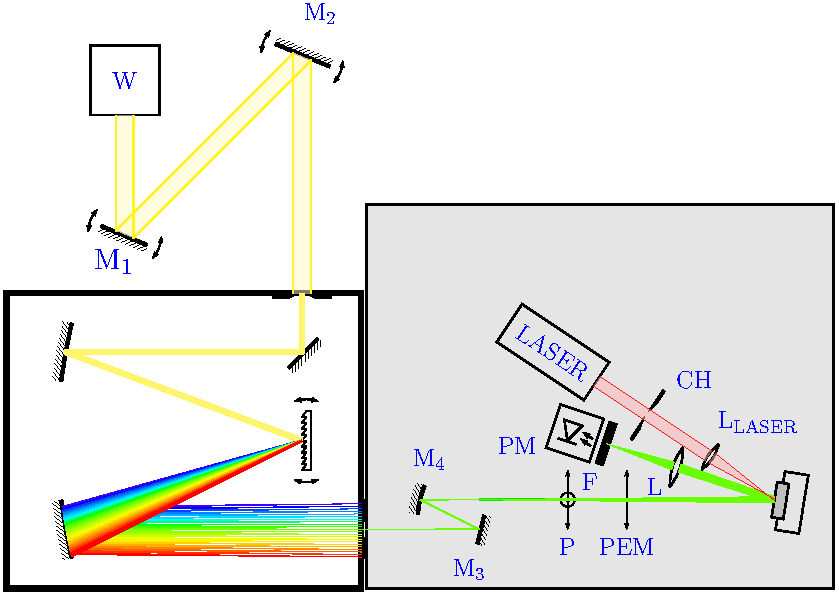
\includegraphics[width=\textwidth]{../figures/chapter-3/pr-setup/build/pr-setup.pdf}
	\caption[PR Scheme]{Photoreflectance setup used in these experiments, the setup implemented is commonly called dark configuration this due that photo-detector are exposed, then keeping closed to ambient light.  W: tungsten lamp, $\mathrm{M_1}$ to $\mathrm{M_4}$ variable mirrors, P: polarizer, PEM: photoelastic modulator, L: focus lens, F: filter, PM: photomultiplier, $\mathrm{L_{LASER}}$: focus lens for laser, CH: mechanical chopper.}
	\label{fig:chapter-3-PR-SETUP}
\end{figure}

The experimental setup to PR experiments implemented in this work, shown in \Cref{fig:chapter-3-PR-SETUP}. The setup start with the probe light from a tungsten lamp, the beam is led by two silver mirrors to monochromator entrance slit, then the monochromatic beam passes through a polarizer and a photoelastic modulator finally affects on sample. The reflected light is focus to the PM with a focus lens. Modulation of the electric field in the sample is caused by photo-excited electron-hole pairs created by the pump source in our case is a red laser that illuminates the same spot of the monochromatic beam and is chopped to a certain frequency, in this setup we use a mechanical chopper at 1KHz. It is important to mention that the reflected light in addition to being  focused by a lens, is filtered before inside at PEM, this is important because the reflected laser light by the sample can modify the modulated R signal, do not forget that the PL signal is involved too. \\*
Although the R signal is modulated by the chopper at 1KHz, after is measure by a lock-in amplifier due to the change in the R is very small about of  $1\times 10^{-4}$,  in comparison with the  PL signal, R change is less than PL as one million times. This is the reason by which any modulated spectroscopy commonly uses a lock-in amplifier. In our case, the setup is called Dark\cite{misiewicz1999photoreflectance} setup because the PM is exposed to room light, therefore the system is keep closed. The  Dark configuration has some advantages, one of these is, that the R changes are subtracted intrinsically therefore the use of the filter is enough to the dispersion of laser is not a problem.  We refer intrinsically to the R signal modulation. If the PL signal achieves to be detected,  the system will perform subtraction as shown in \Cref{eq:chapter-3-PR-mechanis}, if the PL signal mixes with the R in both cases this will cancel because it is constant,  staying only the change in R. 
\begin{figure}[ht!]
	\centering
	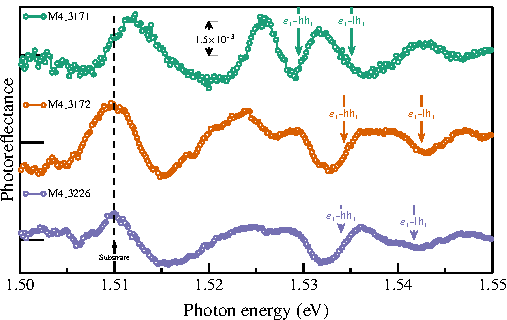
\includegraphics[width=\textwidth]{../figures/chapter-3/pr-plots/build-ruco/pr-set1.pdf}
	\caption{ PR experiments to samples: \sm{3171}, \sm{3172} and \sm{3226} at 30K. Arrows point to calculated transitions for each sample, the used laser wavelength was the same, which in PL experiments and the power used in each of these was 5mW. Dashed line point the GaAs substrate.}
	\label{fig:chapter-3-PR-PLOT-SET1}
\end{figure}

\begin{figure}[ht!]
	\centering
	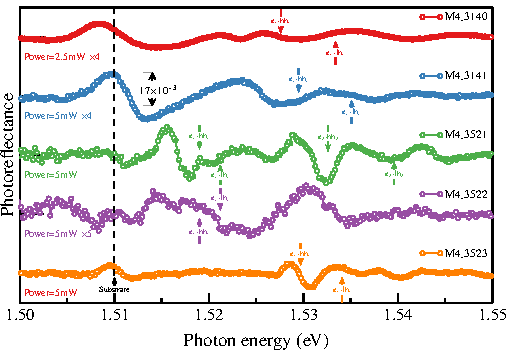
\includegraphics[width=\textwidth]{../figures/chapter-3/pr-plots/build-ruco/pr-set2.pdf}
	\caption{ PR experiments to samples: \sm{3140}, \sm{3141}, \sm{3521}, \sm{3522} and \sm{3523} at 30K. Arrows point to calculated transitions for each sample, the used laser wavelength was the same, which in PL experiments and the previous PR experiments. Dashed line indicate the GaAs substrate, in these samples this transition is well located.  The PR spectra of sample \sm{3522} p-ype doped (orange) is five times smaller  than their correspond n-type, the sample \sm{3521}. The experiments in sample \sm{3140} was performed at 2.5mW, then was multiply it by four in according to samples \sm{3521} and \sm{3523}, in case of the sample\sm{3141} even if,  was performed at a power = 5mW the result was 5 times smaller than sample \sm{3521}. The discussion about of this is explained in the text. }
	\label{fig:chapter-3-PR-PLOT-SET2}
\end{figure}

The result of PR signals associated with band to band and quantum level transitions, in case of samples \sm{43171}, \sm{43172} and \sm{43226} the built-in electric field is low due to the structure n-i-n, this in principle is canceled or screen, this mean that  the field create by carriers is opposite. The \Cref{fig:chapter-3-PR-PLOT-SET1} shows the result of PR experiments on samples mentioned above and are a bit informative. In fact, GaAs gap is not visible in these samples, many mechanisms can affect the PR results in these. The first one and more representative  undoubtedly is the low built-in field, if the structures are n-i-n the field expected is so low although the field can affect the interfaces and contribute but in general this is canceled by opposite photo-carrier directions. Frequently the PR is used tool to calculated or estimate intrinsic fields, this is possible in intermediate-field regimen, this knows as Franz-Keldysh oscillations  (FKOs) by electric field along $z$-direction \cite{shen1995franz}. So, the in PR spectra is observed oscillations and the period is determined by the field in the structure, where typically only about 3-4 FKOs can be detected in the space charge region of a doped sample. In this case for these samples and as will be explained later, the PR experiments are complex in context to determine all transitions  that occur in them and the field is smaller, therefore does not are candidates to have FKOs.

The samples n-i-n type as shown in the \Cref{fig:chapter-3-PR-PLOT-SET1} the FKOs does not exist and this is clearly observable because these experiments does not have any oscillations, as before mentioned this behavior may be occurred because the directions  of photocarriers generated are opposite, then the intrinsic field is canceled. Thus, the PR measured spectra are the result of modulation of intrinsic residual electric field or  nonuniform fields effects\cite{delsole1978effect}.  
In contrast,  with the n-i-n type samples, the i-n type samples exposes clearly the direct transitions even associated to transitions with more energy (next levels energies), although the intrinsic field is not enough to generate FKOs. \\*
In the \Cref{fig:chapter-3-PR-PLOT-SET2} can see the direct transitions numerically calculated for samples \sm{3140}, \sm{3141}, \sm{3521}, \sm{3522} and \sm{3523}. The sample \sm{3521} was taken as reference in terms of amplitude, in the sample \sm{3140} was performed experiments as a function of power laser, being the power 2.5 mW the closest at 5mW, this is one of the reasons for that the result spectra was approx four times smaller than the sample \sm{3521}.   The sample \sm{3522} p-type, maybe can be five times smaller than their n-type analogous sample (\sm{3521}), but the line shape resultant does not have any response, i.e., in terms of amplitude is smaller, but the transitions are not clarified or not resolved. This is one of our keys to final results because it has to do with carrier distribution and the nonexistence of the built-in electric field. For the sample \sm{3141} the PR spectra is similar to the sample  \sm{3140}, the difference between these structures is the barrier width, but in spectra the transitions are more resolved in the sample \sm{3141}.  \\*
\emph{From now on, we focus on the samples :} \sm{3140}, \sm{3521}, \sm{3522} and \sm{3523}, \emph{these samples are similar in structure, if shows experiments of the n-i-n type samples and the rest of i-n type samples is only to remark the importance of our results. }

Even though in many works about the PR is normal to submit a line shape fit model  to clarify the effects of modulated intrinsic fields around of critical points or transitions and as before mentioned this does not the interest of this work. Although, the study and models of line shape for modulated spectroscopy as the PR are essential in the experimental study of semiconductor physics\cite{cardona1969modulation,seraphin1966bandstructure}.  Nevertheless, in our experiments  although the PR mechanism is observable in general around of the Gap ($E_0$) and direct transitions, the mechanism of modulation over the low intrinsic field, exhibit  effects  which is not frequently in the PR experiments, as it is shown in the following section. 


\subsubsection{Excitonic Effects}
\label{subsubsec:chapter-3-PR-exciton-effects}
\vspace{-10mm} 
\lettrine[lines=3, lraise=.1, nindent=0mm, slope=0mm]{\textbf{T}}{he CQWs}, structures are useful to study excitonic effects under external perturbations of an applied electric field. These structures are coupled by the thin barrier, then the electrons overlap over both wells,  this behavior is very studied by the confinement effects and possibility to create combines based on electron properties.  In this work, we focus on the samples which exhibit exciton effects that commonly are observed under external field apply in our case, without external fields or external perturbations and nor any structure modifies\footnote{This refers to create strain by polish over the samples or mechanisms which generates strain, external perturbations also refers to temperature changes, applied currents, and others.} Starting with a comparison between ACQWs n- and p-type these are the \sm{3521} and \sm{3522} samples respectively, \Cref{fig:chapter-3-PR-PLOT-SET3-a)} shows the PR of both samples(left), where the p-type sample is approx five times smaller than the n-type sample, therefore we can conclude that the mechanism of photo-carriers generated in these are different even if it has the same \gls{CQWs} structure.   

\begin{figure}[ht!]
	\centering
\begin{subfigure}{\textwidth}
	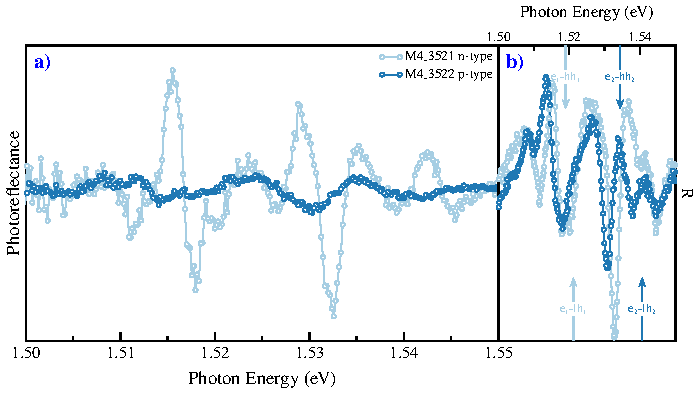
\includegraphics[width=\textwidth]{../figures/chapter-3/pr-plots/build-ruco/pr-set3.pdf}
	\phantomsubcaption\label{fig:chapter-3-PR-PLOT-SET3-a)}
	\phantomsubcaption\label{fig:chapter-3-PR-PLOT-SET3-b)}
\end{subfigure}
	\caption{Comparison of : (a) PR spectra of the 3521 (n-type) and 3522 (p-type) samples, the p-type sample is 5 times smaller than n-type sample. (b) R spectra obtained at same time in each experiment, the arrows point to each direct transitions for two first confined energies. The line shape is practically the same in both spectra.} 
	\label{fig:chapter-3-PR-PLOT-SET3}
\end{figure}


Also, the \gls{R} spectra as shows the \Cref{fig:chapter-3-PR-PLOT-SET3-b)}  obtained synchronously at each experimental measured, this is the DC signal detected by photomultiplier and reading by the multimeter. These signals are practically the same, according to equation \cref{eq:chapter-3-PR-mechanis}  the change originated by the laser source does not enough, i.e., $\Delta R= R_{\mathrm{off}}- R_{\mathrm{on}}$ is smaller. 
In another way, the comparison of samples \sm{3521} (ACQWs-2) and \sm{3523} (SCQWs), shown in the figure \Cref{fig:chapter-3-PR-PLOT-SET4} exhibits the difference in amplitude at same power laser but around de $E_0$ is well resolved in both. In case of the SCQWs sample  the direct transitions are well resolved, but in ACQWs-2 sample, could be present forbidden transitions, pointed at \Cref{fig:chapter-3-PR-PLOT-SET4} with same color of its correspond PR spectra. This behavior it has been observed previously\cite{fox1991excitonic} in MQWs structures even at 300K \cite{shen1986observation}. The nomenclature to allowed transitions  (direct transitions) is: $\thh{\text{n}}{\text{m}}$ for electron-heavy hole and  $\tlh{\text{n}}{\text{m}}$ for electron-light hole, n index represent the n-th conduction subband and m-th  valence subband. So, when n=m its refer to direct transitions or allowed transitions, in ACQWs appear peaks related to transitions between first electron energy where electron wave function is predominantly in the wide well, but this wave function is overlapping to narrow well even if in minor percent, this mean that $\mathrm{n\neq m} $ then the heavy- and light-holes confined at narrow well can create $\thh{1}{2}$,  $\tlh{1}{2}$ transitions, or the electrons in second confined energy that  predominantly  are at narrow well but, they can penetrate (tunneling)   to the  another well (wide well) as seen in   \Cref{fig:chapter-3-PR-PLOT-SET4}  can generate  another forbidden transitions. 
It is important to mentioned that this behavior is presented at low-field regime, therefore can not associate this to modulation of the built-in electric field, this being discussed since some years ago \cite{shen1986observation,shen1987photoreflectance}, even though can this associated, with the behavior which have the  electron, heavy- and light-holes in CQWs structures, with a specific barrier width and the height of the potential barriers  (or depth of wells)\cite{fang1988allowed,sivalertporn2016effectofbarrier}. The electron and holes tunneling depends on those parameters and, in our case, the barriers potential depends on Al percent in the alloy \algaas, therefore $x=0.15$ then the barriers they are not so tall, and the coupling barrier width is very thin ($< 2$ nm). \\
\begin{figure}[ht!]
	\centering
	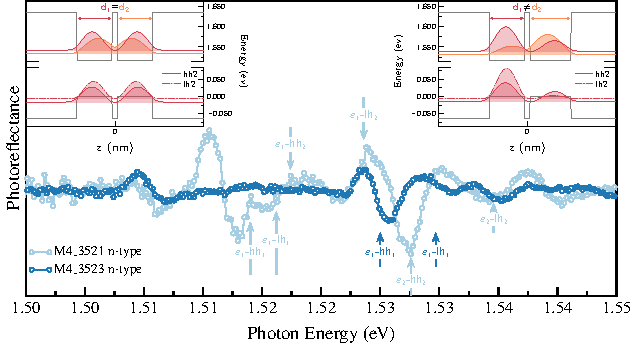
\includegraphics[width=\textwidth]{../figures/chapter-3/pr-plots/build-ruco/pr-set4.pdf}
	\caption{The PR comparison between samples \sm{3521} (ACQWs-2) and \sm{3523} (SCQWs), the electron wave function are plotted  for each sample where, the SCQWs sample at top left and at top right to ACQWs sample. The top arrows pointed to forbidden transitions in  ASQWs-1 sample, while the bottom arrows pointed to the direct transitions in both samples. }
	\label{fig:chapter-3-PR-PLOT-SET4}
\end{figure}

These structures, become an interesting platform to study the phenomenology and behavior of confined electrons, heavy- and light-holes, and their respective interactions. Another interesting phenomenon, which we could observe, was the trions (\xp or \xm) formation through the PR experiments. When were carried out the set of PR experiments over the samples i-n type, occurred a peculiar event while we performed and established the correct measure parameters, to be specific while we determined the laser power. This does not mean that our experiments are wrong, as a matter of fact,  this peculiar event made us test the experimental setup several times and carried out experiments as a function of laser power. This event started with the \sm{3140} (ACQWs-1) sample, this sample has a well with a slightly wide width and because of that the wave function overlapping in major percent than the others samples, by this reason is reasonable or expected, that the trions formation it is more likely as explain later.  While they were being carried out, the PR experiments in ACQWs-1 sample, at higher power laser allowed by our device, in fact, this was trouble, because the laser power does not stable, so it was decided to turn on the laser  previously  before performing each experiment, this was around of eight  hours before to start experiments. After detecting the problem with the laser power, it was tarted the PR experiments at higher laser power, the results were peculiar due to appearing a higher peak with respect to direct transitions, in fact, the direct transitions did not was observable. These experiments were realized several times and the behavior was kept, then we decided to increase the spectral resolution to try to understand the nature of this peak,  previously all experiments were carried out with the  monochromator slits at 1500$\mu$ this to enhance the light collected by PM. The \Cref{fig:chapter-3-PR-PLOT-SET5} shows the evolution of these experiments at P=50mW as a function of the slits aperture, it is clearly that does not about of experimental contraption or another external thing which can contribute or being the cause of this behavior. 
\begin{figure}[h!]
	\centering
	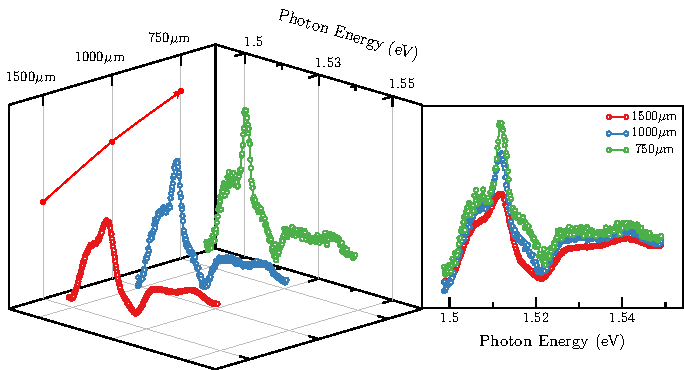
\includegraphics[width=\textwidth]{../figures/chapter-3/pr-plots/build/pr-set5.pdf}
	\caption{PR spectra of the ACQWs-1 sample designed as a function of slits aperture, where it can see the increase of peak resolution as  decrease the aperture of slits.}
	\label{fig:chapter-3-PR-PLOT-SET5}
\end{figure}

From these results it decided all experiments with these apertures of slits, although we  try to enhance the spectra resolutions at 750$\mu$m was they got the best results. In the \Cref{fig:chapter-3-pr-plot-set6}  shows the evolution of the PR spectra as a function of laser power, starting with 1mW of power and finished with 50mW. Remember previously mentioned that the laser power is unstable and this trouble it did not allow performing  the experiments increases power in one way more uniform, this is the reason that the experiments were carried out with powers at 1mW, 3mW, 8mW, 30mW, and 50mW.  The spectra with power less than 8mW are relatively similar, therefore,  after that power it can see a change in peak width and that peak tends to shift at less energy. \\
\begin{figure}[ht!]
	\centering
	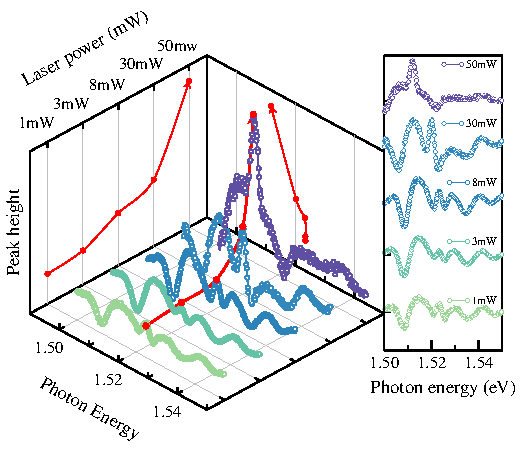
\includegraphics[width=\textwidth]{../figures/chapter-3/pr-plots/build/pr-set6.pdf}
	\caption{The peak tends to height as increase the laser power, which also is very observable as a redshift. }
	\label{fig:chapter-3-pr-plot-set6}
\end{figure}

Now, we establish the physical background of that rare behavior in the PR experiments. In semiconductors, the electron-hole pairs are the reason for many special phenomena and are commonly called the hydrogen atoms in semiconductors. But to understand the nature of excitons and their consequent behaviors, it needs to start with a specific platform to keep or extend their life and interactions.  As above-mentioned, the life of the excitons in QWs is extended for several reasons, of which; well width and low temperatures enhance the binding energy\cite{bastard1982exciton,shinozuka1983wannier}. When the light interacts with these structures, the electron-hole pair associated with the absorption of a photon with enough energy results in an exciton (general explanation), but if inside the structure the electron density is great\cite{kheng1993observation}, the excitons and all possible interactions which can occur as exciton-exciton, exciton-hole (\xm), exciton-electron(\xp), electron-electron, even, LO-phonon-exciton interaction. 
All of this presents in a modification of the line shape resultant, in terms of the PL experiments it is possible to observe unexpected transitions as a slight modification in the line shape. In spite of the physics involved in this mechanism is very complex, the hard work in this theme has generated valuable results. 

Since the 50s Lampert\cite{lampert1958mobile} suggested the existence of charged excitons also called \emph{trions} in semiconductors and after almost 40 years it is proved experimentally\cite{kheng1993observation,stebe1989ground}, and as expected the trions \xp or \xm they were observed in QWs. The electron concentration has a role important in trion formation, for this reason, they usually modulated n- or p-type doping in the QWs structures.  
Also, the external perturbations as the electric\footnote{In this case the trions formation is due a relative position of the Fermi level when the low electric field is applied, in fact, the mechanism involves indirect transitions and is easy that the indirect exciton interact with electrons or holes\cite{yuan2018tunneling}.} or magnetic fields commonly used to enhance the trions transitions, in the magnetic field case, the trions involved acquiring a triplet state nature, so the Zemman splitting is expected, therefore the transitions are well resolved. At zero field, the ground state of trion is a singlet\cite{aceituno2011therole}, this is, two electrons with opposite spin, these electrons are bound with a hole as shows the scheme in \Cref{subfig:chapter-4-trions-scheme-a)}. \\*
\begin{figure}[ht!]
	\centering
	\begin{subfigure}{\textwidth}
		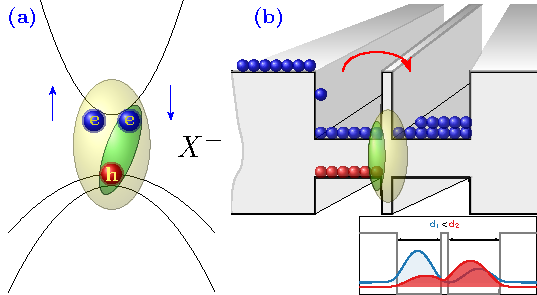
\includegraphics[width=\textwidth]{../figures/chapter-3/trions-scheme/build-ruco/trions-sheme}
		\phantomsubcaption\label{subfig:chapter-4-trions-scheme-a)}
		\phantomsubcaption\label{subfig:chapter-4-trions-scheme-b)}
	\end{subfigure}
	\caption{Trions formation scheme in terms of band structure \subref{subfig:chapter-4-trions-scheme-a)} in this case, the exciton is bound to an electron in the conduction band leading to a three-body system knew as negative trion \xm.  On the other hand, in \subref{subfig:chapter-4-trions-scheme-b)} it presents the possible formation of \xm due to a slight width of one in the CQWS, consequently, the narrow well transfers electrons through tunneling to a wide well, if it is calculated the wave functions of this structure, the wave functions have the characteristic of to be distributed asymmetrically as in the case of the applied electric field along $z$ \cite{sivalertporn2016effectofbarrier,debbar1989coupled}.  }
	\label{fig:chapter-4-trions-scheme}
\end{figure}

In our case, the trions formation is due to photo-excited carriers induced by the laser source, if we suppose that the doped layer is the absolute answer of this, the other samples as SCQWS-1 and ACQWS-2 would have similar results in their PR spectra when it increases laser power, but this is not observed, in fact, in these cases the line shape kept but noisily, then if we adjudicate the trion formation to photo-excited carriers, which is the cause that enables trions in the ACQWs-2 sample?. The answer is a hypothesis that needs extra experiments but is part of the future objectives of this work. The electron and holes (hh, lh) wave functions in samples slightly asymmetric in wells widths, i.e., one of the wells is slightly width than the other, these wave functions have similar behavior as the case when de electric filed is applied. This behavior enhances the electron tunneling from the narrow well to the other well (wide well) as shows in \Cref{subfig:chapter-4-trions-scheme-b)}, if all-important samples contain the doped layer with the same n-type concentration if we suppose that this layer modifies the Fermi level thus generating a small electron gas (2DEG), its possible think that this electron gas has a function of electron reservoir\cite{manassen1996exciton,finkelstein1996negatively}.  Then the photo-carriers generates by the laser source step up carriers dynamics, doing that the narrow well is yielding continuously electrons to wide well through tunneling and, these electrons are recombining with the excitons confined in the plane of the narrow well, therefore results in a three-body system  \xm$=(e,e,h)$ or  \xp$=(e,h,h)$. As it is known, the trion is a charged exciton where the sign depends on its formation, in the case of \xm$=(e,e,h)$  their transition is under the first transition of \xhh, and their energy evolution tends to redshift as can see in \Cref{fig:chapter-3-pr-plot-set6}. Therefore in our case, which was also has been reported 
\cite{sibeldin2001formation,israel2005trions,manassen1996exciton,kheng1993observation,finkelstein1996negatively}, the shift evolution correspond to an \xm trion, however still missing more experiments to strengthen this hypothesis. On the other hand, what happens if the 2DEG does not consider? 
It is very important to emphasize this argument because the objective of this work is to demonstrate that CQWS structures especially ACQWs shows effects of symmetry breaking does not see in structures without external perturbation(application of:  electric or magnetic field,  strain, etc.) or intentional modification (growing of interfaces that unbalance the QWs region, differences in the potential of the barriers), by this reason is importantly empathized that regardless of exist a 2DEG whichever is their electron density and the built-in electric field which can this generate, as a matter of fact,  that field does not represent the cause of the phenomena presented in this work, more later this is discussed with more detail. 
On the other hand, is relatively easy to corroborate that the presence of the electric field on those samples can be regarded as despise, what is the reason to asseverate this if the PR has a principal characteristic the built-in field modulation?
As before mentioned the non-existence of the FKOs is a point to assert the field regime is low, moreover, in comparison with the n-i-n-type samples, also remain in this regime notwithstanding of be designed to reduce the built-in field. However, it is can be estimated by means of \sch-Poisson, so as to, the equation \Cref{eqn:chapter-2-sec-numerical-calculations-schrodinger-discrete} it is coupled Poisson equation\cite{jirauschek2014modeling,harrison2016chap3}
\begin{align}
	\left(\dfrac{d}{dz}\varepsilon(z)\dfrac{d}{dz}\right) V_{p}(z)&=\rho (z)
	\label{eq:chapter-3-poisson-equation-1}\\
	\left(\dfrac{d}{dz}\varepsilon(z)\dfrac{d}{dz}\right) V_{p}(z)&=e\left[n_{\mathrm{D}}(z)-\sum_{i}n_{i}^{s}\left|\psi_{i}(z)\right|^2\right]
	\label{eq:chapter-3-poisson-equation-2}
\end{align}
With the objective of present the behavior and the causes of the high doping in the \algaas layer, we implement a simple code, starting off our numerical codes and helping us with already implemented codes as \gls{aestimo}\cite{hebal2021general},  we calculated numerically \sch-Poisson equation. It is important to mention which solution is self-consistent, therefore the code is implemented with all parameters to divergence avoid,  in our case is due to high doping and this is too large.\\
For this reason, it is inevitable that the codes do not converge, although it can be considered a factor damping to speed convergence\cite{ram2004theschrodinger}.
We consider the damping factor, and we decided to calculate a structure as GaAs/n-type doped \algaas/\algaas, where the width of lateral layers is fixed and the width of the doped layer varies from 15nm to 300 nm with the same n-type doped $6\times 10^{18} \mathrm{cm^{-3}}$.
\begin{figure}[ht!]
	\centering
	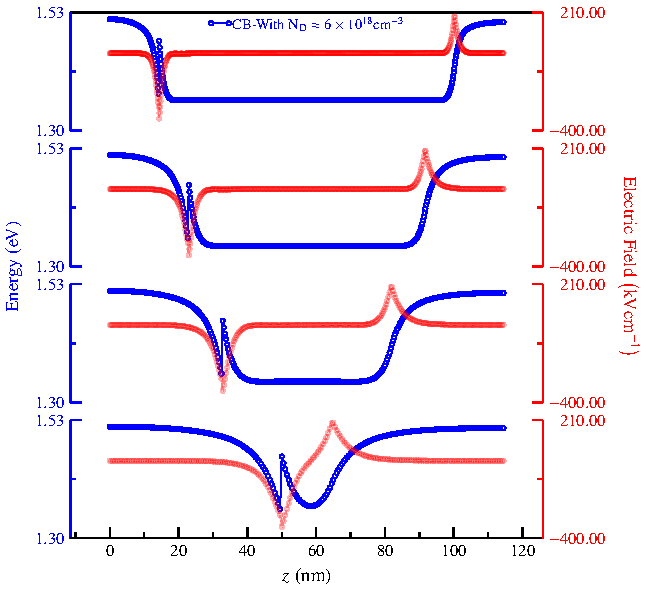
\includegraphics[width=\textwidth]{../figures/chapter-3/poisson/build/poisson.pdf}
	\caption{Results to self-consistently \sch-Poisson equation, in order with down to top the n-type layer $\mathrm{Al_{0.15}Ga_{0.85}As}$ doped ( $6\times 10^{18} \mathrm{cm}^{-3}$) is increasing in width from 15nm, 75nm, 150nm to 300nm. The goal of this is to calculate in a general way the effects of the dopped layer, specifically due to the electric field induced by this.  The strength of the field is expressed in kVcm units, although this magnitude is great, we assume that does not significantly, latter we explained this.}
	\label{fig:chapter-3-pr-poisson-1}
\end{figure}
In general, the self-consistent \sch-Poisson equation, is a process that starts with the calculation of the confined energies in the potential profile defined as $V(z)$,  in this profile are included each parameter of the material that makes up the heterojunction as the doping quantity in each layer if this is doped. After, as shown in \Cref{eq:chapter-3-poisson-equation-2}, is evaluating the space charge with their respective charged donors and their concentration $n_{\mathrm{D}}$,  $n_{i}^{s}$ is the electron sheet density of the confined levels and corresponding wavefunctions $\psi_{i}(z)$. To  calculates the electron density in each level $i$ frequently is applied Fermi-Dirac statistics\cite{cassan2000onthereduction,ando1987calculation,bastard1990wave}. 

This charge distribution in the structure gives rise to space charge effects, resulting in an additional electrostatic potential $V_{p}$ which causes conduction band bending\cite{jirauschek2014modeling,jovanovic2005mechanisms}. The total potential $V$ is the result of $V=V_{0}+V_{p}$, where the $V_{0}$ is the original potential profile, so, this is the iterative part of calculations, in our case, we established the difference between $e_{{1}_{\mathrm{new}}}\! -\! e_{{1}_{\mathrm{old}}}\! <\! 1\times10^{-5}$ as convergence factor. Previously mentioned the damping factor is defined for fast convergence, in our case $\alpha_{\mathrm{damp}}$ is about $1\times 10^{-3}$. The results are shown in \Cref{fig:chapter-3-pr-poisson-1} to a structure :  GaAs/$\mathrm{Al_{0.15}Ga_{0.85}As}$(n-type $6\times 10^{18} \mathrm{cm}^{-3}$)/$\mathrm{Al_{0.15}Ga_{0.85}As}$ with four different widths (15nm, 75nm, 150nm, and 300nm) for the  layer doped. 

\begin{figure}[ht!]
	\centering
	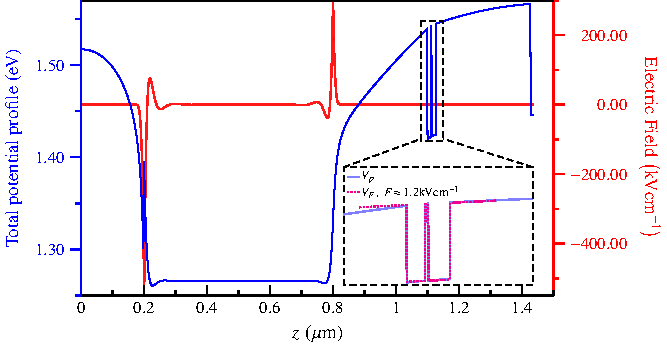
\includegraphics[width=\textwidth]{../figures/chapter-3/poisson/build/poisson-3.pdf}
	\caption{Band conduction profile $V(z)$ calculated by numerical solution of self-consistent Schr\"odinger-Poisson equation. The calculations were performed considering the width of the doped n-type $6\times 10^{18}$ layer with  600nm. The zoom inset shows the comparison between total potential calculated (blue) and when applied field $F\!\approx\! 1.2 \mathrm{kVcm^{-1}}$ (dotted magenta), where at around of CQWs zone are similar.}
	\label{fig:chapter-3-pr-poisson-3}
\end{figure}
In the next chapter, we expose the RAS experiments and their significance in the wonderful results of this work, following, is important to define and explain the role of the doping layer that as can see may be generated a significant intrinsic field which in contrast with the RAS results and our model the built-in electric field does not significatively important in the symmetry breaking ($D_{2} \to C_{2v}$).  Therefore, we calculate the possible conduction band bending due to the built-in electric field as can see in \Cref{fig:chapter-3-pr-poisson-3}.
We have taken into account a total structure width with an n-type doped layer,  we remember that the high doping and large width can cause the calculations does not converge by this we implemented a damping factor to accelerate the convergence, also we calculated a  potential profile considering an external electric field applied around of $F\!\approx\! 1.2 \mathrm{kVcm^{-1}}$. \\*
The results show that practically the total $V_p$ and electric field (line-shape and magnitude) are kept as shown in \Cref{fig:chapter-3-pr-poisson-1}, if we compare the potential profiles $V_{p}$ and $V_{F}$ as see in \Cref{fig:chapter-3-pr-poisson-3}, it can observe that practically the band bending which is generated by electric field so much as by doped layer, as an external field applied are very similar if the external potential is around of $F\!\approx\! 1.2 \mathrm{kVcm^{-1}}$. This means that, if exists an electric field but is comparable with surface field\cite{lastras1999model}, hence is a small field. 
Therefore, we can say that the effects of the trions are associated with the asymmetry of the \gls{QW}s as before mentioned.



 \subsubsection{The PR Summary}
 \label{subsubsec:chapter-3-ps-conclusions}
 \vspace{-10mm}
 In conclusion, the PR remains a powerful tool for experimental solid-state physics, especially in semiconductors study the facility to implement it, and the great information which gives as about fundamental transitions that in comparison with other spectroscopy is still better. Along with the experimental work, we could notice that the PR has the capability of detect behaviors which does not common in this spectroscopy as trions measured, and although this work is still in progress, the satisfaction to propound a novel source to study of an excitonic behavior as the trions,  through easy spectroscopy without external perturbations.  On the other side, the AQCWs has a large potential to study quantum phenomena, especially the interactions and process due to the exciton confined, in this case, something so simple as the relative widths in the CQWs generates a surprising behavior. 



\subsection{Reflectance Anisotropy Spectroscopy (RAS)}
\label{subsec:chapter-3-ras}
 \vspace{-10mm}
\lettrine[lines=3, lraise=.1, nindent=0mm, slope=0mm]{\textbf{T}}{he \gls{RAS}} is the experimental tool that completes the set in this work, without the intention of replicates the physical background and interpretations about RAS, we focus on specific terms to detail our great results.  This spectroscopy, is a  powerful tool in the studying of semiconductors physics, being characterized as default anisotropy study tool.  This experimental technique, was developed by Aspnes\cite{aspnes1973surface,aspnes1985anisotropies, aspnes1985above} to measure \emph{surface-induced} optical anisotropy in cubic semiconductors, although this can be applied around of near-band-edge\cite{wei1995theory}. So, to our purposes, \gls{RAS} is an excellent experimental tool to study optical anisotropies in CQWs structures. In our case both \gls{RAS} and \gls{PR} setup is the same with their exceptions, in the \gls{PR} case is necessary to add the laser to modulated spectroscopy while in the \gls{RAS} the modulation it is realized by the \gls{pem}, which changes the polarization state. As schemes in \Cref{fig:chapter-3-ras-setup}, the monochromatic light first times trough over polarizer prism and the \gls{pem} to finally being focused onto the sample with spot size of 5.00mm diameter. The light reflected by the sample is collected and detected by the multialkali photomultiplier tube (before discussed in \Cref{sec:chapter-3-section-samples-description} and shows in \Cref{tab:chapter-3-section-samples-photodectors-materials}). A detailed description of the RAS technique can be found elsewhere \cite{lflm1993spectrometer}. As shows in \Cref{fig:chapter-3-ras-setup}, the RAS signal is proportional to: 

\begin{equation}\label{eqn:chapter-3-sec-ras-rasequation}
\dfrac{\Delta R}{R} = 2\dfrac{R_{\left[110\right]}-R_{\left[1\overline{1}0\right]}}{R_{\left[110\right]}+
R_{\left[1\overline{1}0\right]}}
\end{equation}

where denotes the orientations $\left[110\right]$ and $\left[1\overline{1}0\right]$ over crystalline directions(see \Cref{fig:chapter-3 GaAs Substrate}). In our experiments the \gls{RAS} signal is around of $10^{-4}$. As well's known if the \gls{RAS} signal it is detected, the structure exhibits an optical anisotropy for in-plane light propagation\cite{koopmans1998microscopic}. The experiments, as the PR case, were it performed at 30K. 

In accordance with \Cref{chap:Chapter-2}, the anisotropy into these structures entails into interesting physical phenomena, overall about of optical properties. This \gls{oa} it is due to the hole mixing, as a long as the structures being under symmetry reduction, in this case from $D_{2d}\to C_{2v}$. If we measured RAS over \gls{SCQWs}, it is expected that this does not exhibit an \gls{oa} or failing that this being smaller due to abrupt interfaces are non-ideal. 
The first part of experiments were carried out over the samples: \sm{3171}, \sm{3172} and \sm{3226},  we remember that these samples are the type n-i-n, this means that they consist in more growth layers, therefore it is expected that the \gls{RAS} signal being smaller. The \Cref{fig:chapter-3-subsec-ras-plots-set-1} shows the results to these samples, in top to bottom order, in left side plots the \gls{RAS} while in right side it is plotted the \gls{R} spectra. The \gls{R} spectra plotted to each sample is the average of all experiments performed, this means which in each \gls{RAS} experiment, the \gls{R} was simultaneously measured, then to each sample it is taking the average.  In order to discuss the result of that samples, we can observe that in general therms these samples gets a smaller signal of \gls{RAS}, although in \gls{R} it does not happen, the direct transitions can being locate in accordance with the numerical results as shows with arrows.
\begin{figure}[H]
	\centering
	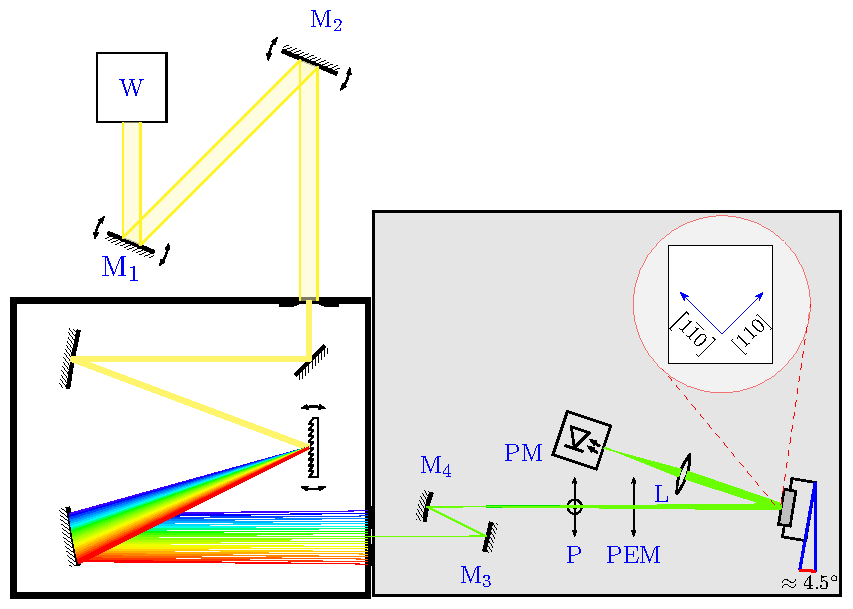
\includegraphics[width=\textwidth]{../figures/chapter-3/ras-setup/build-ruco/ras-setup-2.pdf}
	\caption[RAS Scheme]{RAS setup implemented in this work, as  before explained in the PR  setup, this is a  dark configuration this due that photo-detector are exposed, then keeping closed to ambient light. The optical array is the same as the PR, with the difference which the role of polarization and PEM. This figure also schemes the  incidence angle which is about of $4.5^{\circ}$ and the directions of linear polarization.  }
	\label{fig:chapter-3-ras-setup}
\end{figure}
Although these three samples consists in more several growth layers, it is possible to measure an in-plane anisotropy   were in samples: \sm{3171} and \sm{3226} the signal amplitude it is relatively same in contrast with the sample \sm{3171}.
The first RAS results even they are an asymmetric \gls{CQWs} structures, the  \gls{RAS} spectra it is higher in the samples with AlAs barrier (\sm{3172} and \sm{3226}), then the potential barrier is higher than in the sample \sm{3171}, but the width of these barriers is small, therefore we have a case with samples they consist;  in high coupled barrier and thinner. 
In the other sample, where the \gls{RAS} spectra is smaller (\sm{3171}), the coupled barrier is small in potential in comparison with the other samples, but is more wide. 
\begin{figure}[H]
	\centering
	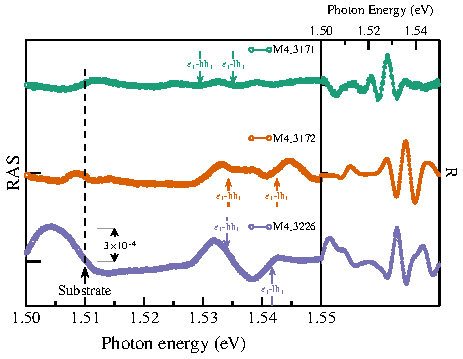
\includegraphics[width=\textwidth]{../figures/chapter-3/ras-plots/build-ruco/ras-set-1.pdf}
	\caption{Experimental results from samples: \sm{3171}, \sm{3172} and \sm{3226}, from top to bottom respectively. In left, shows the RAS result where with a dashed line it is denote the substrate transition, in each sample denotes the direct transitions with arrows. The right side, show the plots of R spectra, which is the average result of all experiments carried in each correspond sample.   }
	\label{fig:chapter-3-subsec-ras-plots-set-1}
\end{figure}
Although, it was  expected that the spectra relatively same in these three samples, the coupled barrier plays an important role this due to the tunneling process,  wells it returns a \gls{RAS} spectra more definite (better line-shape) than the sample with less tunneling, this means, the coupled barrier is wide. Then, the sample \sm{3171} is approx three times smaller. These samples are relatively common with barrier exception, in sample \sm{3226} that  better has \gls{RAS} response posses a coupled barrier with a width of 0.424 nm, while the second with a better RAS response is the sample \sm{3172} which has a barrier width of 0.565 nm.  

In the next set of samples: \sm{3140},  \sm{3141},  \sm{3521},  \sm{3522} and  \sm{3523}, as  is explained in \Cref{sec:chapter-3-section-samples-description}, consists in samples with coupled barrier of \algaasx{0.15}, where the difference in this set samples, is one  of these samples (\sm{43141}) has a coupled barrier  twice wider than the other samples, and the relative width of the wells. 

\Cref{fig:chapter-3-subsec-ras-plots-set-2} shows the results of \gls{RAS} experiments carried out on these samples. These results are interesting in comparison with the before set,  the most notorious is the evolution of \gls{RAS} signal in the more asymmetric structures, in these structures the peaks associated with direct transitions are seen more clearly, being those with an opposite concavity. In these peaks the larger one it is the heavy-hole (down concavity) while the  smaller one it is the light-hole transition (up concavity). It is totally evident that the samples \sm{3521} and \sm{3522} (also called as ACQWs-1 and ACQWs-2) exhibits great \gls{RAS} response, then, in  accordance with the model anisotropy  has a major hole mixing.  Also, the \gls{R} spectra is well resolved in both samples, with a peculiarity in the transitions concavities, which in both, is up concavity. 
\begin{figure}
	\centering
	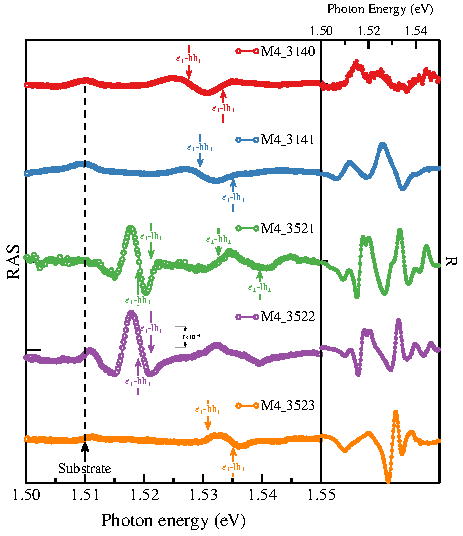
\includegraphics[width=\textwidth]{../figures/chapter-3/ras-plots/build-ruco/ras-set-2.pdf}
	\caption{Experimental results from samples: \sm{3140}, \sm{3141}, \sm{3521}, \sm{3522} and \sm{3523}, from top t bottom respectively. In left, shows the RAS result where with a dashed line it is denote the substrate transition, in each sample remarks the direct transitions with arrows. The right side, show the plots of the R spectra, which is the average result of all experiments carried in each correspond sample. Also, it is denote the \gls{RAS} magnitude proportional to $7\times 10^{-4}$, which in contrast with \gls{SCQWs} samples the signal is smaller. The direct transitions  it is locate by two peaks with opposite concavity where can see that the larger one transition is $\thh{1}{1}$  and  smaller one associated with the $\tlh{1}{1}$.}
	\label{fig:chapter-3-subsec-ras-plots-set-2}
\end{figure}
\subsubsection{RAS strength discussion and the physical model justification}
\label{subsubsec:chapter-3-ras-discussed}
\vspace{-10mm}
To enter into discussion, it purpose is to focus on the three samples before mentioned, aiming to expose the principal objective of this work, which is denoted the \gls{RAS} strength in \gls{ACQWs} as importance in the  optical properties and excitonic effects in these structures. The \Cref{fig:chapter-3-subsec-ras-plots-set-3} exposes the evolution of \gls{RAS} strength, in this plot it is indisputable that the signal increases, because the comparison between the three samples where it is starting with a symmetric structure, then with a lightly asymmetric structure and finally with a very asymmetric structure, the \gls{RAS} signal associated with each transition have opposite concavities and redshift as the structure is more asymmetric. \\*
Due to the fact that the wave-function probability density of sample \gls{SCQWs} is distributed symmetrically along the QW
structure, the \gls{oa} strength is expected to be similar to that
obtained for a single \gls{QW}. In fact, a \gls{RAS} signal of the order of magnitude of $0.1\times 10^{-3}$ has been reported for an 8 nm single \gls{QW} \cite{chen2002interface}, which has the same order of magnitude as the spectra of \Cref{subfig:chapter-3-subsubsec-ras-strength-set-3-c}. This \gls{oa} is attributed to the inequivalent AlGaAs/GaAs interfaces along the \gls{SCQWs}
structure. It is important every clear the role of tunneling in the coupled wells, the difficulty to get a model to explain this structures  does not it the same as the single QW structure.  \\
As pointed out before (\Cref{subsec:chapter-2-anisotropy-model}), the strength of the \gls{oa} signal is produced by an intermixing of the heavy- and light-hole states in the valence band that is proportional to  $\mel{\psi_{\mathrm{hhn}}}{\cal{H}}{\psi_{\mathrm{lhn}}}$ according to \Cref{eqn:chapter-2-sec-anisotropy-model-perturbative}. For the lowest heavy- and light-hole levels
(n = 1), there is an estimated separation in energy of around $\Delta E_1 = 2.0$, 4.1, and 4.4 meV for samples \gls{ACQWs}-2 (\gls{ACQWs}-3), \gls{ACQWs}-1, and \gls{SCQWs}, respectively. The mixing $\mel{\psi_{\mathrm{hhn}}}{\cal{H}}{\psi_{\mathrm{lhn}}}$ can be estimated by considering that the transitions are direct (n is the same for the valence and conduction band) and then the overlapping terms in \Cref{eqn:chapter-2-sec-anisotropy-model-perturbative} must be approximately the same for each sample.  For transitions $n=1$ it can be seen in \Cref{fig:chapter-3-subsec-ras-plots-set-3} that amplifier ratios of the spectra between ACQWs-2 and ACQWs-1 with respect to SCQWs are 1.5 and 3.7, respectively.  Thus from \Cref{eqn:chapter-2-sec-anisotropy-model-perturbative} we estimate ratios of  $\mel{\psi_{\mathrm{hh1}}}{\cal{H}_{\mathrm{ACQWs-1}}}{\psi_{\mathrm{lh1}}}/\mel{\psi_{\mathrm{hh1}}}{\cal{H}_{\mathrm{SCQWs}}}{\psi_\mathrm{lh1}}\sim 1.4$  for sample \gls{ACQWs}-1 and $\mel{\psi_{\mathrm{hh1}}}{\cal{H}_{\mathrm{ACQWs-2}}}{\psi_{\mathrm{lh1}}}/\mel{\psi_{\mathrm{hh1}}}{\cal{H}_{\mathrm{SCQWs}}}{\psi_\mathrm{lh1}}\sim 1.7$ for sample \gls{ACQWs}-2.
\begin{figure}[H]
	\floatbox[{\capbeside\thisfloatsetup{capbesideposition={right,top},capbesidewidth=0.4\textwidth}}]{figure}[0.95\FBwidth]
	{\caption{RAS spectra for the \subref{subfig:chapter-3-subsubsec-ras-strength-set-3-a}, \subref{subfig:chapter-3-subsubsec-ras-strength-set-3-b}, asymmetric and \subref{subfig:chapter-3-subsubsec-ras-strength-set-3-c} symmetric CQWs. The dashed vertical line indicates the expected energy of the excitonic transition of the GaAs substrate. Above this energy, the optical transitions come from the CQWs. The inset shows the PL spectra measured for each sample. Two peaks can be identified in each spectrum, a larger one associated with the transition $\thh{1}{1}$ and a much smaller one associated with the $\tlh{1}{1}$ (for spectrum \subref{subfig:chapter-3-subsubsec-ras-strength-set-3-b} this peak is observed as a shoulder). The energies obtained from the PL spectra are indicated by the arrows in the RAS spectra. Note that the structures associated with $\thh{1}{1}$ and $\tlh{1}{1}$ increase their strength when the CQWs become more asymmetric. The RAS spectra were measured at 30 K.
	}\label{fig:chapter-3-subsec-ras-plots-set-3}}
	{
	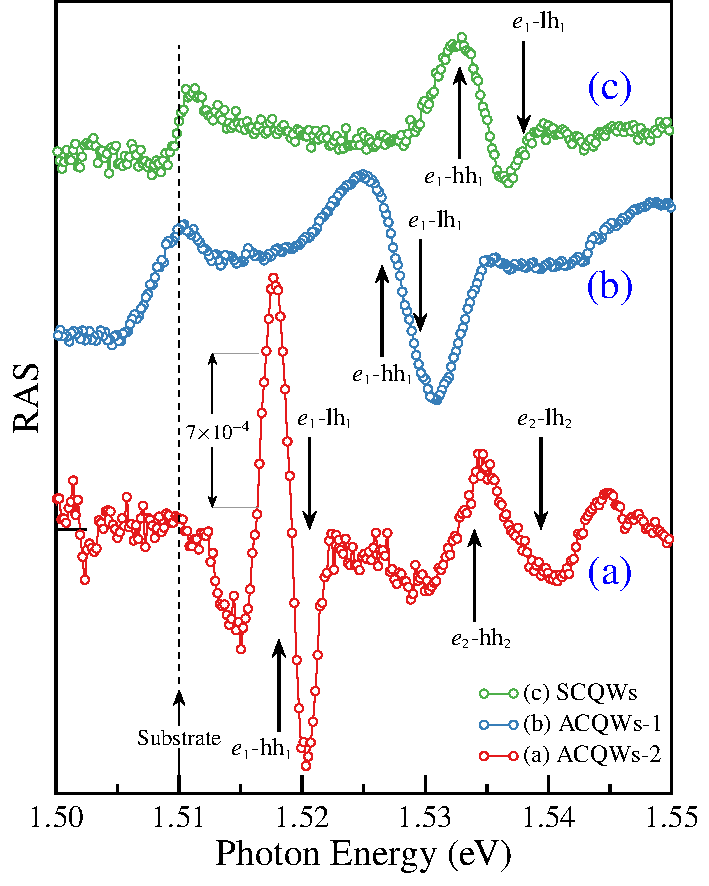
\includegraphics[width=0.6\textwidth]{../figures/chapter-3/ras-plots/build-ruco/ras-set-3.pdf}
	\phantomsubcaption\label{subfig:chapter-3-subsubsec-ras-strength-set-3-a}
	\phantomsubcaption\label{subfig:chapter-3-subsubsec-ras-strength-set-3-b}
	\phantomsubcaption\label{subfig:chapter-3-subsubsec-ras-strength-set-3-c}
	}
\end{figure}
In accordance with our estimation based on the anisotropy model, the \Cref{tab:sec-chapter-3-ras-table} contains the energies considered. If well, the large \gls{oa}  in general, it is attributed to interfaces in our case the reason is due to non-equivalence due to the width asymmetric into coupled QWs, this originates a mixing of hh-lh states and therefore these it coupled strongest as the states close in energy\cite{winkler2003spin}. The \Cref{tab:sec-chapter-3-ras-table} and \Cref{fig:chapter-2-sec-numerical-calculations-results} confirms this, in the ACQWs-2 this energy between $\mathrm{hh_1}$ and $\mathrm{lh_1}$ states are close, in counterpart with the  SCQWs  this energy is large.\\

\begin{table}[t]
	\centering
	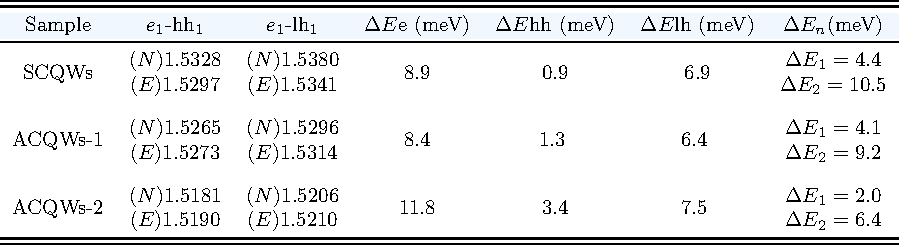
\includegraphics[width=\textwidth]{../tables/chapter-3/table-ras/build-ruco/table-ras.pdf}
	\caption{Comparative of experimental (E) and numerical calculations (N) of first level transition  energies (in eV). $\mathrm{\delta Ee}$, $\mathrm{\delta Ehh}$ and $\mathrm{\delta Elh}$ corresponds to the difference between electrons, heavy- light holes states, respectively. $\mathrm{\Delta E_n}$ is the numerical calculation of energy splitting for transitions 1 and 2 ($ \mathrm{n}=1,2$).}
	\label{tab:sec-chapter-3-ras-table} 
\end{table}
\begin{figure}
	\floatbox[{\capbeside\thisfloatsetup{capbesideposition={left,top},capbesidewidth=0.4\textwidth}}]{figure}[0.95\FBwidth]
	{\caption{Reflection anisotropy (RAS, \subref{subfig:chapter-3-subsubsec-ras-strength-set-4-a}, \subref{subfig:chapter-3-subsubsec-ras-strength-set-4-b} ) and differential reflection (DR, solid line) spectra for ACCQWs-2 and ACQWs-3,  grown on an AlGaAs n-type  and  p-type layer respectively. Note that while for the heavy hole transitions ($\thh{1}{1}$ and  $\thh{2}{2}$) in the RAS and DR spectra have the same concavity, for light holes transitions ($\tlh{1}{1}$ and  $\tlh{2}{2}$) the concavities are opposite and DR spectra shows the highest level transitions. The bottom arrows point to the experimental transitions for the two first levels, whereas the top arrows show the calculated energies to three energy levels.  The RAS and DR spectra were measured at 30K.}\label{fig:chapter-3-subsec-ras-plots-set-4}}
	{
	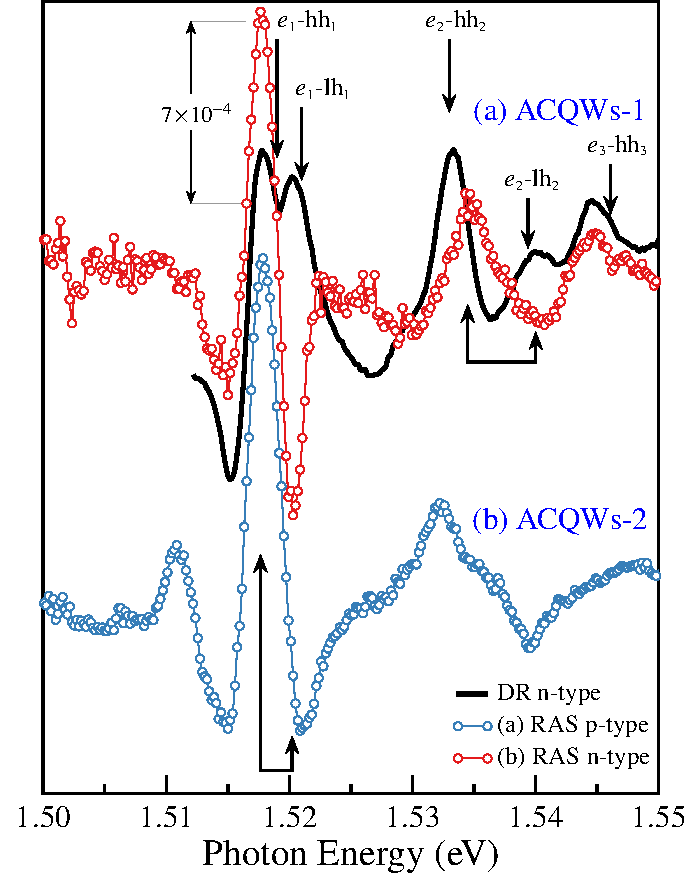
\includegraphics[width=0.6\textwidth]{../figures/chapter-3/ras-plots/build-ruco/ras-set-4.pdf}
	\phantomsubcaption\label{subfig:chapter-3-subsubsec-ras-strength-set-4-a}
	\phantomsubcaption\label{subfig:chapter-3-subsubsec-ras-strength-set-4-b}
	}
\end{figure}
\begin{figure}
	\floatbox[{\capbeside\thisfloatsetup{capbesideposition={right,top},capbesidewidth=0.4\textwidth}}]{figure}[0.95\FBwidth]
	{ \caption{RAS experiment designed to demonstrate the non-existence of built-in electric field trough sequential measured along the preferential direction, in this case, it was chosen  along the pits $[1\overline{1}0]$\cite{weyher2010defect}. The signal result in both samples practically is the same, the sign is conserving. At top left and right located the images taken with a microscope of back substrate which shows the pit reveals along of $[1\overline{1}0]$ direction. 
	}\label{fig:chapter-3-subsec-ras-orientation}}
	{
	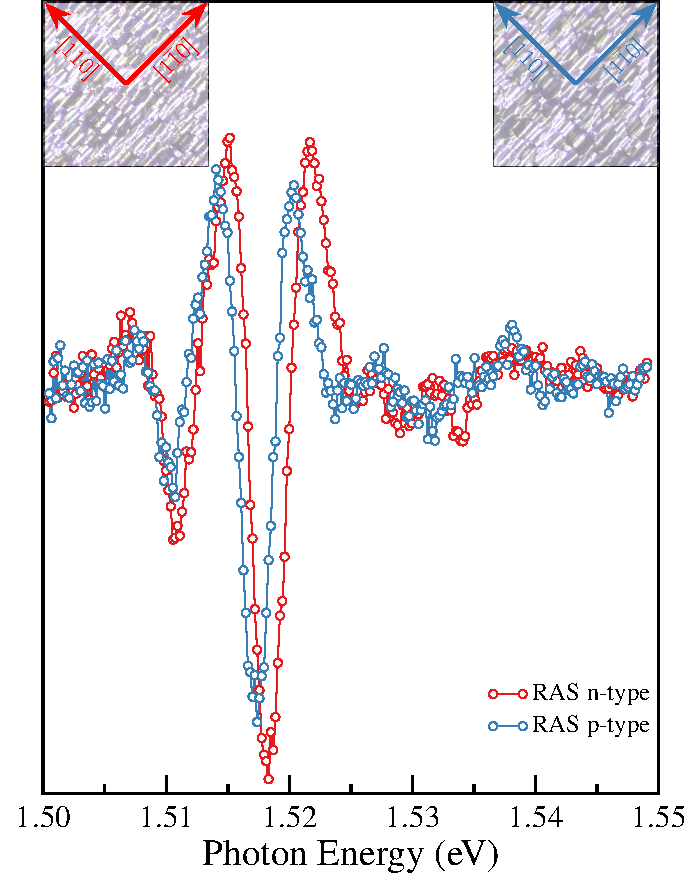
\includegraphics[width=0.6\textwidth]{../figures/chapter-3/ras-plots/out/ras-set-5.pdf}
	}
\end{figure}

In order to elucidate the physical origin of the RAS in the \gls{ACQWs}, we compare in \Cref{fig:chapter-3-subsec-ras-plots-set-4} the RAS and the DR spectra of the \gls{ACQWs}-2. DR spectra is obtained by the numerical subtraction of the reflection (\gls{R}) spectra recorded at 30K and 300K followed by the normalization to the 300K spectrum. The subtraction highlights the excitonic features, which are very weak (and energy shifted) at 300K. The comparison between RAS and DR spectra allows us to contrast the contribution of the heavy and light holes transitions. Around 1.5175 eV, the DR spectrum shows two peaks corresponding to  $\thh{1}{1}$ and  $\tlh{1}{1}$ transitions. Note that in the RAS spectrum, the structure associated to $\thh{1}{1}$ transition has the same concavity as the corresponding for the DR spectrum, while the  $\tlh{1}{1}$ transition has the opposite concavity. This  is an indication of the transfer of oscillator strength between the levels due to the intermixing of heavy- and light- holes, thus supporting our anisotropy model. The same behavior applies for the $\thh{2}{2}$ and $\tlh{2}{2}$ transitions at around 1.5375 eV. Transition  $\thh{2}{3}$ is also indicated and it has the same concavity for RAS and DR spectra, as in the case of the $\thh{1}{1}$ and  $\thh{2}{2}$ transitions.
The arrows at the bottom of \Cref{fig:chapter-3-subsec-ras-plots-set-4} indicate the energy of the states $\thh{\text{n}}{\text{n}}$ and $\tlh{\text{n}}{\text{n}}$ (for n =1 and 2) obtained from the  maximum and minimum of the RAS spectrum. 
From the numerical calculation results summarized in  \Cref{tab:sec-chapter-3-ras-table}, the energy splitting between transitions  $\thh{\text{n}}{\text{n}}$ and  $\tlh{\text{n}}{\text{n}}$  are $\mathrm{\Delta E_1}=2.0$ meV and $\mathrm{\Delta E_2}=6.4$ meV. In accordance with \Cref{eqn:chapter-2-sec-anisotropy-model-perturbative}, the \gls{oa} amplitude is proportional to $1/\mathrm{\Delta E_n}$. Considering the same valued for the overlapping and the mixing $\mel{\psi_{\mathrm{hhn}}}{\cal{H}}{\psi_{\mathrm{lhn}}}$ we estimate an amplitude ratio of 3.25 between these transitions. This value is close to the value of 3.9 obtained by the RAS spectrum of \Cref{fig:chapter-3-subsec-ras-plots-set-4} supporting our interpretation.

Finally, we discuss the possible contribution to the RAS amplitude by a built-in electric field across the CQWs both symmetric and asymmetric. To study this contribution, we have compared the RAS spectra of asymmetric samples \gls{ACQWs}-2 and \gls{ACQWs}-3. The difference between them is the doping of the AlGaAs layer (see \Cref{tab:chapter3:Samples description}). While for \gls{ACQWs}-2 it is n-type, for \gls{ACQWs}-3 it is p-type. Assuming that the built-in electric field  originates from charge transfer between surface states and  the AlGaAs doped layer (n or p), this field is expected to have opposite signs for samples \gls{ACQWs}-2 and \gls{ACQWs}-3. Thus, the linear contribution of the electric field to the \gls{RAS} should be reversed in sign for such samples. \Cref{fig:chapter-3-subsec-ras-orientation} shows the comparison between the \gls{RAS} spectra of samples \gls{ACQWs}-2 and \gls{ACQWs}-3,  this with aim to demonstrate that  in the case of existed a field the sign is opposite.    The experiment, it was designed to measure both samples in a sequence way along the same preferential direction, in this case we choose the direction of pits $\left[1\overline{1}0\right]$ \cite{weyher2010defect}, if existed a field we expected a opposite RAS signal, but this does not occur, the sign in signal it was conserved in both samples. The \Cref{fig:chapter-3-subsec-ras-orientation} shows the results of this experiment, in top left and right it is placed the images of both samples of the pits orientation, this to corroborate that the direction of measured. 
As can be seen (\Cref{fig:chapter-3-subsec-ras-plots-set-4}), RAS spectra are equivalent in shape and have the same sign, thus indicating that the contribution of the electric field to the \gls{RAS} signal is very small. \\

It is natural to suppose that the built-in electric field contributes to increase of the \gls{RAS} signal, and although  we estimate that this field is small, it is still important to discussed it and show different ways to affirms that  the built-in field is not the reason of the \gls{oa}. 
We conclude, thus, that the dominant contribution to \gls{RAS} spectra is the asymmetry of the \gls{CQWs} system. 

\subsubsection{The RAS summary}
\label{subsubsec:chapter-3-ras-conclusions}
\vspace{-10mm}
In conclusion, the RAS proofs experimentally that the \gls{oa} increases as a degree of asymmetry in \gls{CQWs} structures. This behavior is attributed to the reduction of the symmetry of the electronic states in the \gls{CQWs} with \gls{QW}s of different thicknesses. The nature of the transitions was identified by
using PL spectroscopy and numerical calculations. We believe
that the results presented in this work are important and will
be useful in understanding the evolution of the optical transition induced by the breakdown of translation symmetry in asymmetric CQWS.










